\typeout{NT FILE STATE-ART.tex}%
\chapter{Background and Related Work}%
\label{ch:state-art}
%
\begin{quote}
\begin{flushright}
``\emph{We stand on the shoulders of giants.}'' \\
\textbf{-- Isaac Newton}, mathematician, physicist, astronomer
\end{flushright}
\end{quote}

This chapter establishes the technical context for the thesis. We begin with mixed-criticality systems (\glspl{mcs}): why they matter, where they appear, and the challenges they pose for timing predictability, isolation, and assurance under practical \gls{swap-c} constraints. We then outline the current approach to manage this complexity, highlighting the trade-offs they introduce.
%
Next, we survey \glspl{uav}' reference hardware and software
stacks, covering both open-source and commercial solutions, with emphasis on
properties relevant to mixed-critical deployments (e.g., platform support,
determinism, and isolation).
%
Finally, we review related work, organized recent research along the axes most
pertinent to this thesis (flight stacks, onboard platforms, and
virtualization). This positions the contribution that follows and clarifies the
specific gaps the proposed design addresses.

\section{Mixed Criticality Systems}%
\label{sec:mixed-crit-syst}
Embedded platforms increasingly host many functions on the same hardware to
reduce size, weight, power, and cost (\gls{swap-c})~\cite{burns2022mixed}.
However, not all functions are equally critical. In safety-regulated domains,
strong guarantees are required to ensure that consolidation does not compromise
safety~\cite{burns2022mixed,davis_mixed_2018}.
%
Standards such as ISO~26262~\cite{iso26262} and DO-178C~\cite{sc_167_software_1992}
formalize these assurances, particularly in automotive and avionics.
On the one hand, consolidation pressures favor efficient resource sharing to
minimize \gls{swap-c}; on the other hand, domain isolation is needed to
guarantee non-interference. The fundamental question in \glspl{mcs} is how to
reconcile these conflicting goals -- providing strong separation for assurance
while enabling sharing for efficiency~\cite{burns2022mixed}. Addressing this
requires system designs that integrate software and hardware on a single
platform, together with modeling, verification, and, where applicable,
certification~\cite{davis_mixed_2018,youn_software_2015}.

A \gls{mcs} is, simply, a system that integrates software components of two or
more criticality levels on the same platform~\cite{davis_mixed_2018}. Consider a
\gls{uav} executing a video-surveillance mission
(Fig.~\ref{fig:mcs-example}). Tasks are color-coded by criticality according to
DO-178C~\cite{sc_167_software_1992,youn_software_2015}. Navigation and stability
are life-critical: flight-control loops must meet their deadlines under all
conditions, or catastrophic failure may occur. Accordingly, sensor acquisition,
communication handling, processing, and actuation must complete within
predefined time bounds. Here, \emph{criticality} denotes the assurance level
required to bound the probability of such
failures~\cite{sc_167_software_1992,youn_software_2015}.

\begin{figure}[!hbtp]
  \centering
  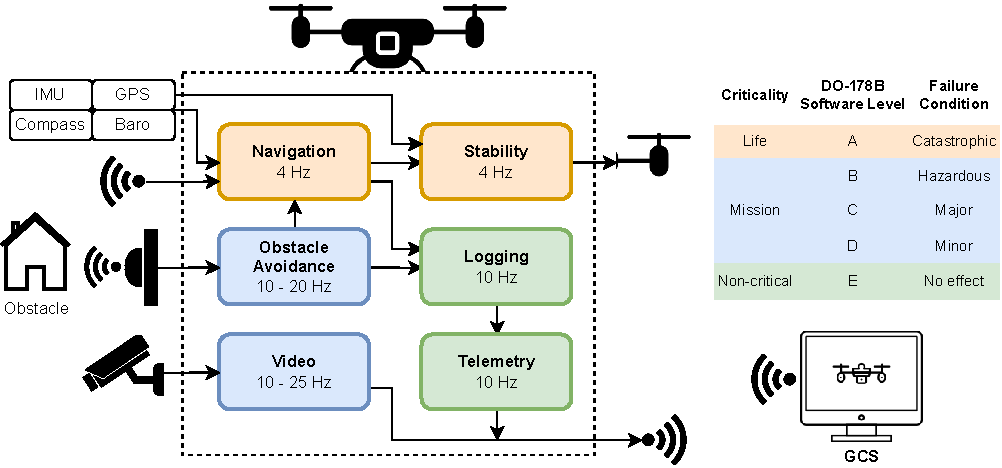
\includegraphics[width=1.0\textwidth]{./img/pdf/mcs-example}
  \caption[Mixed-criticality system example: UAV application]{Mixed-criticality system example: UAV application (adapted from~\cite{yip_relaxing_2014}).}%
  \label{fig:mcs-example}
\end{figure}

By contrast, obstacle avoidance and video capture are mission-critical. They
have soft real-time requirements, but their consequences differ: failing to
detect an obstacle may endanger the aircraft, whereas dropping camera frames is
generally acceptable. Lastly, auxiliary tasks such as logging and telemetry are
non-critical, as missing soft deadlines does not cause safety harm.

One consequence of applying the DO-178C safety standard at a system level is that all \gls{uav}
functions would need to be developed to the life-critical level of navigation
and stability~\cite{youn_software_2015,davis_mixed_2018}. In our case, that
would make ``missing a camera frame'' as unlikely -- and as costly to assure -- as
``missing an actuator output'', resulting in substantial over-engineering of
mission- and non-critical subsystems. The alternative is to demonstrate
\emph{temporal and spatial isolation}, i.e., that lower-assurance functions can
neither delay nor corrupt higher-assurance functions, even under
faults~\cite{cinque2022virtualizing,davis_mixed_2018}.

While \gls{mcs} principles apply broadly, \glspl{uav} face domain-specific
hurdles. They must meet extreme \gls{swap-c} limits: (1) every gram of weight
counts, especially in lower weight classes~\cite{alladi2022UAVBlockain}, affecting the \gls{uav}'s autonomy
and flight dynamics; (2) they operate in uncontrolled,
rapidly changing environments~\cite{faical_adaptive_2017}; (3) and must maintain critical functions during faults, since not every error can be
anticipated~\cite{mohsan2022towards}.
The
shift to mainstream multicore architectures further complicates resource
sharing~\cite{burns2022mixed}. Current approaches reveal a core trade-off: on
one hand, multi-board designs provide strong isolation but poor \gls{swap-c}
metrics; on the other, single-board designs improve \gls{swap-c} but weaken isolation.

Two major research branches stem from this dichotomy. A more \emph{theoretical}
line studies scheduling with criticality-dependent \glspl{wcet} to schedule
systems at each criticality level, but at the cost of higher processor utilization~\cite{lee_estimating_2023}. A more \emph{practical}
line focuses on safe partitioning with shared computational and communication
resources, at the cost of increased design complexity~\cite{cinque2022virtualizing}. Combining the two is
hard as flexible scheduling typically requires at least dynamic partitioning,
whereas certified systems favor complete separation or static
partitioning~\cite{burns2022mixed}. This gap is acute in \glspl{uav}, where both
efficiency and assurance are non-negotiable.

\subsection{Virtualization}%
\label{sec:virtualization}
Mixed-criticality systems integrate software of disparate criticality on shared
hardware. As noted above, the most promising practical approach is to partition
the system safely while sharing compute resources. This leads to the concept of
\emph{virtualization}: a logical abstraction of hardware with isolation
guarantees, realized via hypervisors, \gls{os}-level virtualization, or
unikernels~\cite{cinque2022virtualizing}.
%
Fig.~\ref{fig:virt-mindmap} maps the key concepts referenced in this section,
and Fig.~\ref{fig:virt-approaches-exs} illustrates representative
approaches~\cite{cinque2022virtualizing}. Starting on the left, a conventional
software stack runs an \gls{os} (with runtime and libraries) directly on the
hardware and hosts applications. In this model, failures in any component can
propagate system-wide because no isolation layer intervenes.

\begin{figure}[!hbtp]
  \centering
  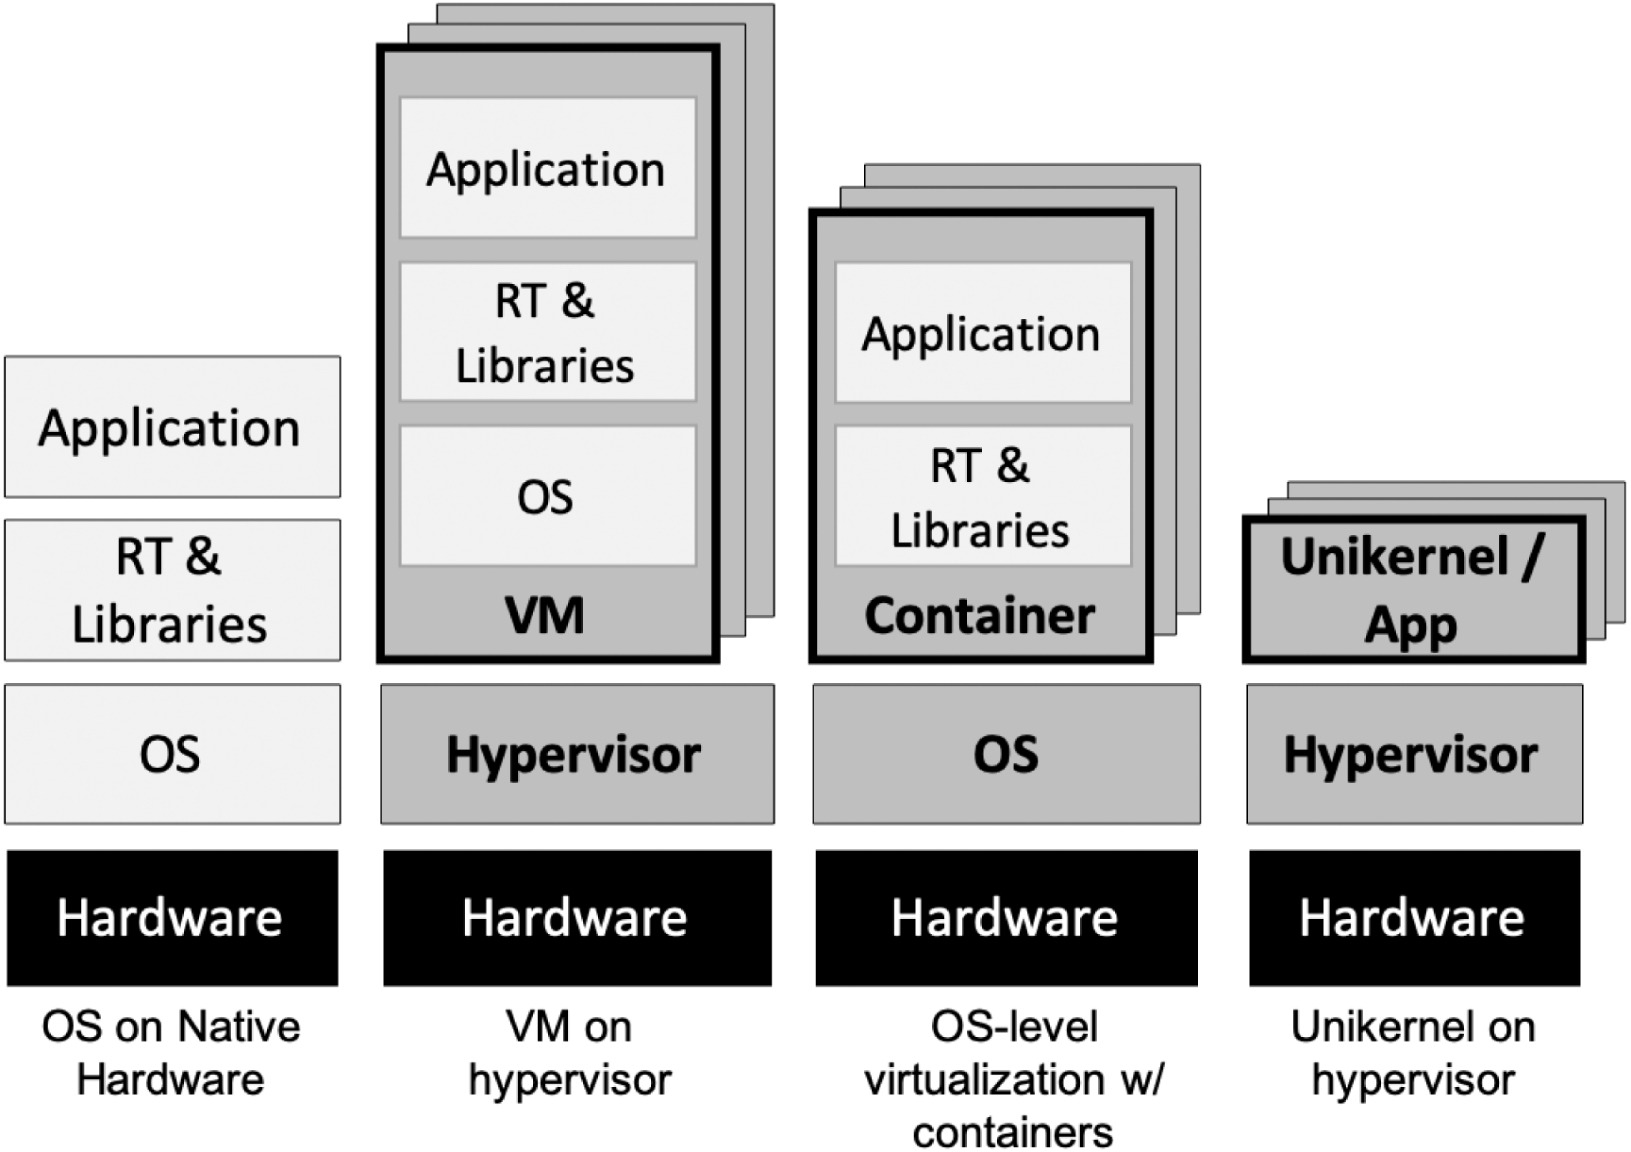
\includegraphics[width=0.6\textwidth]{./img/jpg/virt-approaches-exs} 
  \caption[Examples of virtualization approaches]{Examples of virtualization approaches~\cite{cinque2022virtualizing}\footnotemark}%
  \label{fig:virt-approaches-exs}
\end{figure}
%
\fnlicReq{Elsevier}{5457890117132}%

Next is hypervisor-based virtualization, which inserts a software layer that
abstracts hardware resources so that multiple isolated application
environments -- \glspl{vm} or guests -- can run on the same
machine~\cite{cinque2022virtualizing}. Hypervisors are detailed in the next
section.

\gls{os}-level virtualization (containerization) does not emulate hardware.
Popularized by Docker~\cite{sollfrank_evaluating_2021,kumar_economically_2016},
it is widely used in cloud settings to avoid replicating the full \gls{os} stack
and to increase consolidation~\cite{cinque2022virtualizing}. A container is a
process-like domain atop the host \gls{os}, with isolated namespaces and managed
resources (\gls{cpu}, memory, filesystem, network)~\cite{cinque2022virtualizing}.
Although it lacks hardware emulation, containerization is gaining traction in
\gls{rt} contexts~\cite{xilinxRunX,struhar2020real} and in \gls{uav} systems to
deploy user-space applications on mission computers~\cite{auterion-sw-services}.
Trade-offs include sources of non-determinism (e.g., dynamic resource
assignment), large trusted code bases, and limited hardening, which complicate
testing, assurance, and certification~\cite{cinque2022virtualizing}.

Finally, unikernel-based virtualization compiles the entire software stack
(minimal \gls{os} components, libraries, language runtime, and application) into
a single \gls{vm} image -- a unikernel or library \gls{os} -- that typically runs atop
a general-purpose hypervisor~\cite{cinque2022virtualizing}. Unikernels offer
fast boot, low memory footprint, high performance, and strong isolation (via the
host hypervisor), but reduce flexibility: applications must target the unikernel
environment. Further work is needed for \glspl{mcs}, particularly regarding
certification and dependability support~\cite{cinque2022virtualizing}.

Cinque et al.~\cite{cinque2022virtualizing} relate hypervisor/guest-\gls{os}
pairings to typical use cases. General-purpose (non-\gls{rt}) hypervisors host
non-\gls{rt} guests for server consolidation, and can host \gls{rt} guests for
functional testing and prototyping (without hard guarantees). Real-time
hypervisors host non-\gls{rt} guests for \gls{qos}/performance studies and \gls{rt}
guests for safety-critical workloads. \glspl{mcs} sit in this latter space: they
require a real-time hypervisor capable of hosting both \gls{rt} and non-\gls{rt}
guests with strong isolation and bounded interference. We therefore examine
hypervisors next.

Before proceeding, we briefly clarify a related trend in the telecommunications
domain often called \emph{softwarization}, which occasionally appears under the
umbrella of virtualization~\cite{pathak_uav_2020,liu_deep_2022,nogales_adaptable_2018}.
Softwarization implements network functions that historically resided in
hardware appliances (routers, firewalls, etc.) as software running on
general-purpose servers under \glspl{vm} or
containers~\cite{kumari_taxonomy_2020}. These software instances are termed
\emph{virtual network functions} (e.g., virtual firewalls, virtual
routers)~\cite{cotroneo_nfv-bench_2017}.
%
Softwarization is also gaining traction in the \gls{uav}
field~\cite{sara_softwarization_2016,pathak_uav_2020,siddiki_abir_software-defined_2023,oubbati2020softwarization},
supporting network-centric architectures, service deployment, and communication
management, especially as systems evolve toward multi-\gls{uav}
coordination~\cite{li_distributed_2024,azari_uav--uav_2020}. However, it targets
non-critical networking stacks and thus falls outside the scope of our analysis.

\subsection{Hypervisors}%
\label{sec:superv--hyperv}
A hypervisor is a \glsxtrfull{vmm}: a software layer that abstracts hardware so
multiple isolated application environments -- \glspl{vm} or guests -- can run on
the same machine (see Fig.~\ref{fig:virt-approaches-exs}). Each \gls{vm}
typically includes a guest \gls{os} and its applications. To be useful in
mixed-criticality settings, the hypervisor must enforce temporal, spatial, and
fault-containment isolation~\cite{cinque2022virtualizing}. \emph{Temporal isolation} means a task in one
virtual domain must not cause harmful delays to tasks in another. \emph{Spatial}
(memory) isolation refers to separating code, data, and device access between
domains, generally using hardware protection (e.g., \gls{mmu}, \gls{iommu}). \emph{Fault
containment} ensures that errors do not propagate to block or crash the entire
system.

Hypervisors are commonly classified by where they run, how guests interact with
them, and whether they provide explicit real-time support. \emph{Bare-metal} (type~I)
hypervisors run directly on hardware and control resources themselves (e.g.,
Jailhouse~\cite{jailhouse}, Bao~\cite{martins_et_al:OASIcs:2020:11779},
CLARE~\cite{clare-home}, Xen~\cite{xen-home}).%
\footnote{Xen is typically classified as type~I (bare metal)~\cite{cinque2022virtualizing}.}
\emph{Hosted} (type~II) hypervisors run atop a host \gls{os} and manage resources
indirectly (e.g., KVM~\cite{kivity2007kvm}). In \emph{full virtualization} the
guest runs unmodified while the hypervisor emulates or traps privileged operations (e.g.,
KVM, Hyper-V~\cite{microsoftHyperV}); in \emph{paravirtualization} the guest
cooperates with the hypervisor via hypercalls (e.g., Xen~\cite{barham2003xen}).
\emph{Real-time} hypervisors add mechanisms to allocate and police time budgets so \glspl{vm}
meet timing constraints~\cite{cinque2022virtualizing}. These can be \emph{dynamic}
(resources assigned at run time; e.g., KVM~\cite{kivity2007kvm}, Xen~\cite{barham2003xen})
or \emph{static} (resources fixed at instantiation; e.g., Jailhouse~\cite{jailhouse}, Bao~\cite{martins_et_al:OASIcs:2020:11779}),
with static designs often preferred for \glspl{mcs} due to lower overhead, smaller
code bases, and simpler testing/certification~\cite{cinque2022virtualizing}. Hypervisors also vary by
application scope, from embedded/mission-specific to general-purpose~\cite{heiser2008role}.

Solution families reflect these choices~\cite{cinque2022virtualizing}. \emph{Separation-kernel}
hypervisors implement a small bare-metal partitioning layer that defines fixed
\glspl{vm} and information flows, delegating rich \gls{os} services and drivers to
guests (e.g., PikeOS~\cite{pikeOS}, Xtratum~\cite{masmano2009xtratum}, Jailhouse~\cite{jailhouse},
Bao~\cite{martins_et_al:OASIcs:2020:11779}). \emph{Microkernels} implement only minimal abstractions and
operations in supervisor mode (e.g., memory and thread management, \gls{ipc}), placing
drivers and higher-level services in user mode; some can serve as a hypervisor
with a user-level \gls{vmm} (e.g., seL4 with CAmkES \gls{vmm}~\cite{klein_sel4_2009,matos_sel4_2022}).
These approaches differ in emphasis: microkernels structure an \gls{os} from small user-mode components atop a minimal kernel; separation kernels
focus on static partitioning and isolation -- often leveraging hardware
virtualization -- and rely on guests for \gls{os}-like functionality~\cite{cinque2022virtualizing}.%

General-purpose hypervisors (e.g., KVM, Xen) can be extended with real-time
features. Some approaches leverage security \gls{cpu} extensions (e.g., Arm
TrustZone, Intel SGX) to strengthen isolation, albeit with platform dependence
(e.g., LTZVisor/RTZVisor~\cite{pinto2016towards,rtzvisor}, VOSYSMonitor~\cite{lucas2017vosysmonitor,lucas_vosysmonitor_2018}).
Unikernel solutions package a single application with minimal \gls{os} services
to run atop a hypervisor (e.g., ClickOS~\cite{martins2014clickos},
HermitCore~\cite{lankes2016hermitcore}), trading flexibility for fast boot, small footprint, and performance.

In practice, selection is guided by footprint, alignment with safety standards,
licensing, fault tolerance, security,
and hardware coverage~\cite{cinque2022virtualizing}. Cinque
et~al.~\cite{cinque2022virtualizing} provide a broad survey of such solutions in the context of \glspl{mcs}
and industrial requirements.

\subsubsection{Bao}%
\label{sec:bao}
\emph{Bao} (Mandarin ``bǎohù'', ``to protect'') is an open-source, lightweight,
security- and safety-oriented bare-metal hypervisor for embedded real-time
\glspl{mcs}, developed by the ESRGv3 team at the University of
Minho~\cite{martins_et_al:OASIcs:2020:11779,baoRepo}. It follows the static,
type-I partitioning model popularized by \emph{Jailhouse}~\cite{jailhouse} but
removes the Linux host dependency, thereby reducing the system
\gls{tcb} -- currently \(\sim 8\,\text{kLOC}\) of C plus \(\sim 500\,\text{LOC}\) of
assembly -- and easing the path toward
certification~\cite{martins_et_al:OASIcs:2020:11779}. Bao supports Armv7/8-A,
Arm-R, and RISC-V (RV32/RV64), with ongoing work toward Infineon TriCore and
Renesas RH850.

Bao is a clean-slate design (Fig.~\ref{fig:bao-arch}) comprising a thin,
privileged layer that leverages \gls{isa} virtualization for static
partitioning~\cite{martins_et_al:OASIcs:2020:11779}. It has no scheduler and
does not rely on external libraries or a privileged \gls{vm} (e.g., Linux),
in contrast to Jailhouse~\cite{jailhouse}; instead, it depends only on standard
platform-management firmware to initialize the system and perform
platform-specific tasks~\cite{martins_et_al:OASIcs:2020:11779}. Removing the
Linux dependency improves safety/security posture and real-time
behavior~\cite{martins_et_al:OASIcs:2020:11779}.

\begin{figure}[!hbtp]
  \centering
  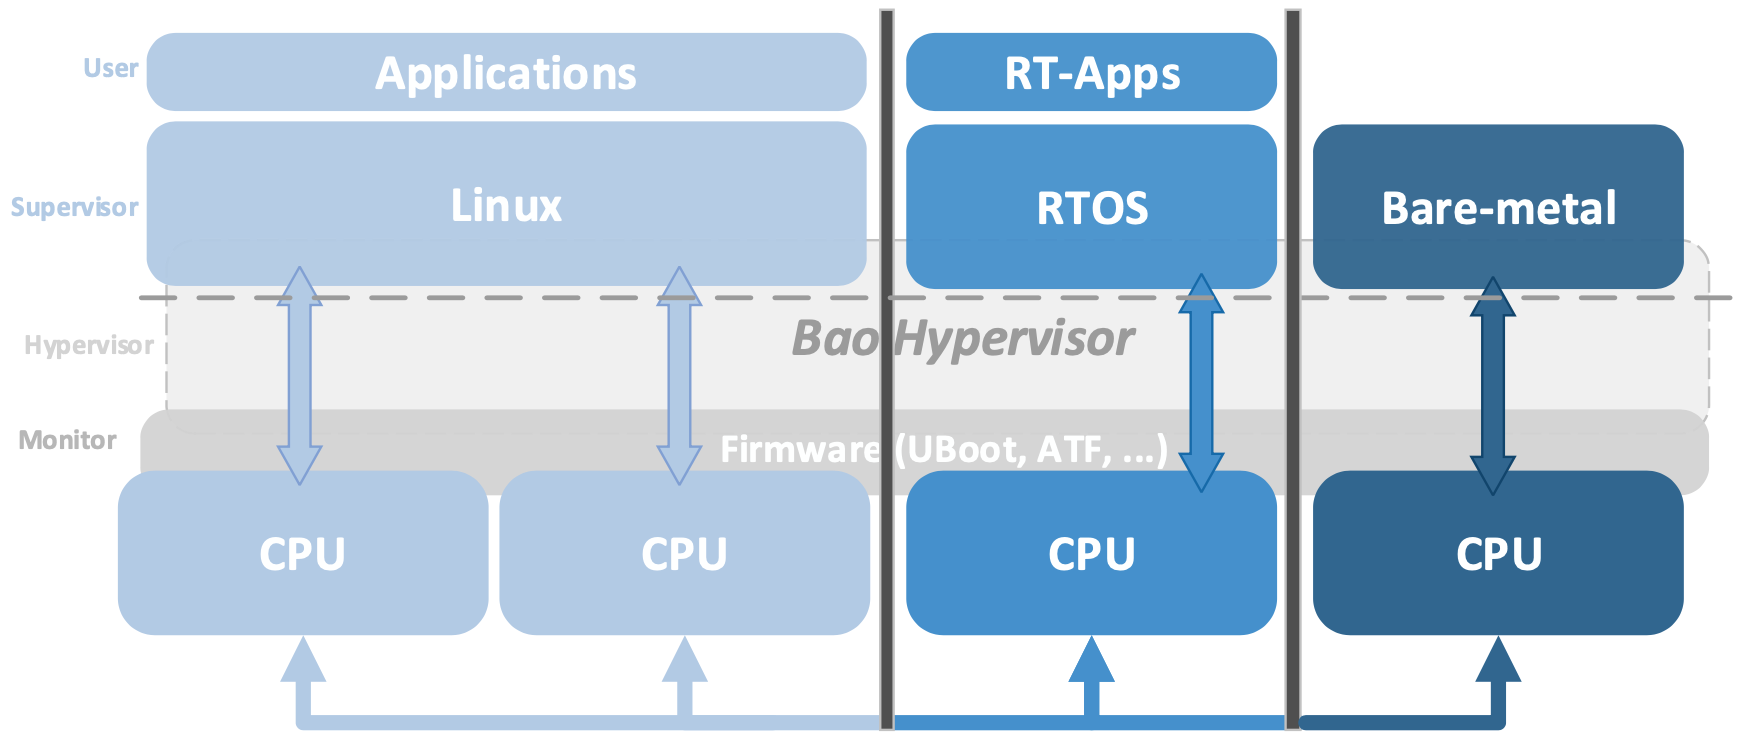
\includegraphics[width=0.7\textwidth]{./img/png/bao-arch}
  \caption[Bao hypervisor architecture]{Bao hypervisor architecture~\cite{martins_et_al:OASIcs:2020:11779}\footnotemark}%
  \label{fig:bao-arch}
\end{figure}
\fnlicCC{foot:bao-embedded-world-lic1}%

Bao targets safety-critical systems by providing temporal, spatial, and
fault-containment isolation~\cite{martins_et_al:OASIcs:2020:11779}. \emph{Temporal isolation}
follows from the absence of a scheduler and the exclusive 1:1 mapping between
virtual and physical \glspl{cpu} at \gls{vm} instantiation time, together with
guest access to per-\gls{cpu} architectural timers~\cite{martins_et_al:OASIcs:2020:11779}.
\emph{Spatial isolation} is ensured by statically assigned memory enforced via
two-stage translation, using superpages when possible to reduce translation and
\gls{tlb} pressure and to aid speculative fetch~\cite{martins_et_al:OASIcs:2020:11779}.
While these mechanisms provide strong isolation and predictable timing,
shared hardware resources (e.g., \glspl{llc}, interconnects, memory
controllers) can still induce temporal interference and expose \glspl{vm} to
\gls{dos} and timing side channels~\cite{bansal2018evaluating,barham2003xen,ge2018survey}.
To mitigate these effects, Bao supports cache coloring for \gls{llc}
partitioning and memory-bandwidth regulation~\cite{martins_et_al:OASIcs:2020:11779}.

For devices, Bao favors direct assignment (pass-through). For memory-mapped
\gls{io}, the same two-stage translation used for memory protection applies;
exclusivity is not enforced automatically, so deployments must avoid unintended
sharing~\cite{martins_et_al:OASIcs:2020:11779}. Paravirtualized I/O via
\emph{VirtIO} is available for selected
devices~\cite{costa2022virtio,ribeiro2023virtio,rocha_mitigating_2023,peixoto-virtio-2024,baoRepo},
enabling efficient sharing while preserving isolation and complementing
pass-through where appropriate. Bao also offers inter-\gls{vm}
communication via shared
memory~\cite{martins_et_al:OASIcs:2020:11779,baoEmbeddedWorld2020}.
%
Interrupt virtualization currently targets Arm \gls{gic}v2/v3, which route
interrupts to the hypervisor for re-injection, adding latency and code
complexity~\cite{martins_et_al:OASIcs:2020:11779}. Arm \gls{gic}v4 addresses
this with direct guest delivery~\cite{arm-gicv4,dall2018design}, though adoption
remains limited. On RISC-V, Bao supports both the legacy \gls{plic} and the more
recent \gls{aia}~\cite{marques_interrupting_2024,baoRepo}.

Relative to alternatives (e.g., Xen’s Dom0-less mode), Bao offers a similar
static-partitioning model with a smaller \gls{tcb} and a clean security posture,
with minimal virtualization
overhead~\cite{martins_et_al:OASIcs:2020:11779}. It has been extensively
benchmarked with the MiBench \gls{aics} suite for real-time embedded domains,
showing low overheads and demonstrating that cache coloring, although not
optimal, can effectively mitigate inter-\gls{vm}
interference~\cite{martins2023shedding}.

Overall, Bao is a strong foundation for a trustworthy, open-source reference
software stack for \gls{uav} applications: it is open-source, enforces strict
domain isolation with efficient resource sharing, and has undergone extensive
benchmarking, enabling consolidation of mixed-criticality software on a single
hardware platform while minimizing \gls{swap-c}.%
Table~\ref{tab:bao-summary} presents a concise summary of Bao’s properties.


% \begin{table}[!hbtp]
%   \caption[Bao hypervisor summary]{Bao hypervisor summary~\cite{baoRepo}}

% Please add the following required packages to your document preamble:
% \usepackage{multirow}
% \usepackage{graphicx}
% \usepackage[table,xcdraw]{xcolor}
% Beamer presentation requires \usepackage{colortbl} instead of \usepackage[table,xcdraw]{xcolor}
% Please add the following required packages to your document preamble:
% \usepackage{multirow}
% \usepackage{graphicx}
% \usepackage[table,xcdraw]{xcolor}
% Beamer presentation requires \usepackage{colortbl} instead of \usepackage[table,xcdraw]{xcolor}
\begin{table}[!hbtp]
\caption[Bao hypervisor summary]{Bao hypervisor summary~\cite{baoRepo}}
\label{tab:bao-summary}
\resizebox{\columnwidth}{!}{%
\begin{tabular}{lllll}
\hline
{\color[HTML]{000000} \textbf{Architecture}} &
  {\color[HTML]{000000} \textbf{Supported platforms}} &
  {\color[HTML]{000000} \textbf{Size}} &
  {\color[HTML]{000000} \textbf{License}} &
  {\color[HTML]{000000} \textbf{Version}} \\ \hline
{\color[HTML]{000000} \begin{tabular}[c]{@{}l@{}}Type I,\\ Static\end{tabular}} &
  {\color[HTML]{000000} \begin{tabular}[c]{@{}l@{}}Armv7/8-A, Armv7/8-R\\ RISC-V RV32 and RV64\\ Infineon Tricore 1.8 (WIP)\\ Renesas RH850 (WIP)\end{tabular}} &
  {\color[HTML]{000000} \begin{tabular}[c]{@{}l@{}}Small \\ $\sim$8 kLOC C +\\ $\sim$500 LOC ASM\end{tabular}} &
  {\color[HTML]{000000} Apache 2.0} &
  {\color[HTML]{000000} 1.0} \\ \hline
{\color[HTML]{000000} \textbf{Features}} &
  \multicolumn{4}{c}{{\color[HTML]{000000} \textbf{Isolation}}} \\ \hline
{\color[HTML]{000000} Static partioning} &
  \multicolumn{2}{l}{{\color[HTML]{000000} \textbf{Spatial}}} &
  \multicolumn{2}{l}{{\color[HTML]{000000} \textbf{Temporal}}} \\ \cline{2-5} 
{\color[HTML]{000000} IO pass-through and VirtIO support} &
  \multicolumn{2}{l}{{\color[HTML]{000000} }} &
  \multicolumn{2}{l}{{\color[HTML]{000000} }} \\
{\color[HTML]{000000} \begin{tabular}[c]{@{}l@{}}1:1 mapping of virtual to physical CPUs \\ (no scheduler required)\end{tabular}} &
  \multicolumn{2}{l}{\multirow{-2}{*}{{\color[HTML]{000000} \begin{tabular}[c]{@{}l@{}}Provided by a 2-stage translation \\ HW virtualization support\end{tabular}}}} &
  \multicolumn{2}{l}{\multirow{-2}{*}{{\color[HTML]{000000} \begin{tabular}[c]{@{}l@{}}Exclusive CPU assignment \\ discards the scheduler\end{tabular}}}} \\
{\color[HTML]{000000} \begin{tabular}[c]{@{}l@{}}Virtual interrupts directly mapped \\ to physical ones\end{tabular}} &
  \multicolumn{2}{l}{{\color[HTML]{000000} }} &
  \multicolumn{2}{l}{{\color[HTML]{000000} }} \\
 &
  \multicolumn{2}{l}{{\color[HTML]{000000} }} &
  \multicolumn{2}{l}{{\color[HTML]{000000} }} \\
 &
  \multicolumn{2}{l}{{\color[HTML]{000000} }} &
  \multicolumn{2}{l}{{\color[HTML]{000000} }} \\
\multirow{-3}{*}{\begin{tabular}[c]{@{}l@{}}No external dependencies (except for \\ standard platform management firmware)\end{tabular}} &
  \multicolumn{2}{l}{\multirow{-5}{*}{{\color[HTML]{000000} \begin{tabular}[c]{@{}l@{}}Translation overhead is minimized using \\ superpages whenever possible, faciliting \\ speculative fetch for potential guest \\ performance improvement\end{tabular}}}} &
  \multicolumn{2}{l}{{\color[HTML]{000000} }} \\
{\color[HTML]{000000} } &
  \multicolumn{2}{l}{{\color[HTML]{000000} }} &
  \multicolumn{2}{l}{{\color[HTML]{000000} }} \\
\multirow{-2}{*}{{\color[HTML]{000000} \begin{tabular}[c]{@{}l@{}}Provides a basic mecanism for inter-VM \\ communication\end{tabular}}} &
  \multicolumn{2}{l}{{\color[HTML]{000000} }} &
  \multicolumn{2}{l}{{\color[HTML]{000000} }} \\
{\color[HTML]{000000} } &
  \multicolumn{2}{l}{{\color[HTML]{000000} }} &
  \multicolumn{2}{l}{{\color[HTML]{000000} }} \\
\multirow{-2}{*}{{\color[HTML]{000000} \begin{tabular}[c]{@{}l@{}}State-of the art partioning mechanisms to \\ be implemented (e.g., memory throttling)\end{tabular}}} &
  \multicolumn{2}{l}{\multirow{-4}{*}{{\color[HTML]{000000} \begin{tabular}[c]{@{}l@{}}It uses cache coloring to enable LLC cache \\ partioning independently for each VM, but \\ at the expenses of memory waste and \\ fragmentation and increased boot time\end{tabular}}}} &
  \multicolumn{2}{l}{\multirow{-8}{*}{{\color[HTML]{000000} \begin{tabular}[c]{@{}l@{}}Per-CPU architecture timers \\ are available to and directly \\ managed by the guests\end{tabular}}}} \\ \hline
{\color[HTML]{000000} \textbf{IO}} &
  \multicolumn{2}{l}{{\color[HTML]{000000} \textbf{Interrupts}}} &
  \multicolumn{2}{l}{{\color[HTML]{000000} \textbf{Related Work}}} \\ \hline
{\color[HTML]{000000} } &
  \multicolumn{2}{l}{{\color[HTML]{000000} }} &
  \multicolumn{2}{l}{{\color[HTML]{000000} }} \\
{\color[HTML]{000000} } &
  \multicolumn{2}{l}{{\color[HTML]{000000} }} &
  \multicolumn{2}{l}{{\color[HTML]{000000} }} \\
\multirow{-3}{*}{{\color[HTML]{000000} \begin{tabular}[c]{@{}l@{}}Directly assigned to guest in a \\ pass-through only IO configuration\end{tabular}}} &
  \multicolumn{2}{l}{\multirow{-3}{*}{{\color[HTML]{000000} \begin{tabular}[c]{@{}l@{}}Supports Arm GICv2 and GICv3\\ Supports RISC-V PLIC and AIA\end{tabular}}}} &
  \multicolumn{2}{l}{\multirow{-3}{*}{{\color[HTML]{000000} \begin{tabular}[c]{@{}l@{}}Jailhouse: pioneer in the static \\ partioning adopted by Bao but \\ requires the Linux Kernel to boot\end{tabular}}}} \\
{\color[HTML]{000000} } &
  \multicolumn{2}{l}{{\color[HTML]{000000} }} &
  \multicolumn{2}{l}{{\color[HTML]{000000} }} \\
{\color[HTML]{000000} } &
  \multicolumn{2}{l}{{\color[HTML]{000000} }} &
  \multicolumn{2}{l}{{\color[HTML]{000000} }} \\
{\color[HTML]{000000} } &
  \multicolumn{2}{l}{{\color[HTML]{000000} }} &
  \multicolumn{2}{l}{{\color[HTML]{000000} }} \\
{\color[HTML]{000000} } &
  \multicolumn{2}{l}{{\color[HTML]{000000} }} &
  \multicolumn{2}{l}{{\color[HTML]{000000} }} \\
\multirow{-5}{*}{{\color[HTML]{000000} \begin{tabular}[c]{@{}l@{}}For memory-mapped IO it uses the existing \\ memory mechanism and 2-stage translation \\ provided by the virtualization support\end{tabular}}} &
  \multicolumn{2}{l}{\multirow{-5}{*}{{\color[HTML]{000000} \begin{tabular}[c]{@{}l@{}}Interrupts are forwarded to the hypervisor \\ which must re-inject them in the VM using \\ a limited set of pending registers\end{tabular}}}} &
  \multicolumn{2}{l}{\multirow{-5}{*}{{\color[HTML]{000000} \begin{tabular}[c]{@{}l@{}}Xen Dom0-less: eliminates the \\ Linux dependency to boot and \\ execute\end{tabular}}}} \\
{\color[HTML]{000000} } &
  \multicolumn{2}{l}{{\color[HTML]{000000} }} &
  \multicolumn{2}{l}{{\color[HTML]{000000} }} \\
{\color[HTML]{000000} } &
  \multicolumn{2}{l}{{\color[HTML]{000000} }} &
  \multicolumn{2}{l}{{\color[HTML]{000000} }} \\
{\color[HTML]{000000} } &
  \multicolumn{2}{l}{{\color[HTML]{000000} }} &
  \multicolumn{2}{l}{{\color[HTML]{000000} }} \\
{\color[HTML]{000000} } &
  \multicolumn{2}{l}{{\color[HTML]{000000} }} &
  \multicolumn{2}{l}{{\color[HTML]{000000} }} \\
\multirow{-5}{*}{{\color[HTML]{000000} \begin{tabular}[c]{@{}l@{}}Paravirtualized I/O via VirtIO is supported \\ for selected devices, enabling efficient \\ sharing with isolation\end{tabular}}} &
  \multicolumn{2}{l}{\multirow{-5}{*}{{\color[HTML]{000000} }}} &
  \multicolumn{2}{l}{\multirow{-5}{*}{{\color[HTML]{000000} \begin{tabular}[c]{@{}l@{}}Bao provides basically the same \\ features from the previous ones, \\ but has a smaller TCB and \\ implements clean security features\end{tabular}}}} \\ \hline
\end{tabular}%
}
\end{table}

\section{Unmanned Aerial Vehicles}%
\label{sec:unmann-aeri-vehicl}
\glsxtrfull{uav}, \glsxtrfull{uas} or, more commonly, \emph{drones}, are unmanned
robotic aircraft capable of executing missions and carrying payloads, guided
either by remote control stations or autonomously~\cite{alladi2022UAVBlockain,glossner2021overview}.
They belong to a broader class of \glspl{uv}, alongside \glspl{ugv}, \glspl{usv}
(e.g., boats), and \glspl{uuv}~\cite{glossner2021overview}.

\glspl{uav} date back as far as the 18\textsuperscript{th} century: in 1783,
France publicly demonstrated the first uncrewed aircraft -- a hot-air
balloon~\cite{uavHistory}. In 1896, Alfred Nobel reportedly launched a
camera-equipped rocket, and in 1935 the first modern radio-controlled aircraft
was developed in the U.K.~\cite{uavHistory}. The term \emph{drone} is often
attributed to Lieutenant Commander Delmer Fahrney, who was in charge of the U.S.
Navy’s \emph{Radio Controlled Aircraft} program~\cite{uavHistory}. A \gls{uav}
designed for surveillance and scouting was developed in Israel in 1973, and the
\emph{Gulf War} marked the first conflict with significant \gls{uav}
use~\cite{uavHistory}. Commercial momentum accelerated in the 2000s, with
civilian permissions arriving in the U.S. in 2006; smartphone-controlled
quadcopters appeared around 2010, and consumer camera drones reached the market
by 2013~\cite{uavHistory}.

Open-source autopilot projects amplified accessibility and capability:
Paparazzi UAS (2003)~\cite{paparazzi-home}, ArduPilot (2008)~\cite{arduPilotHistory},
and Dronecode/PX4 (2011)~\cite{px4History}. Prices dropped as ecosystems grew,
fueling a commercial boom. In North America, UAV market revenue reached
\$737\,millions in 2017, with forecasts of roughly \$6.7\,billions by 2026, driven by
agriculture, security, and law enforcement~\cite{mohsan2022towards}.
%
\gls{uav} versatility spans high-value tasks often difficult or unsafe for humans~\cite{silvagni_multipurpose_2017,lammers_airborne_2023}:
search and rescue~\cite{silvagni_multipurpose_2017}, precision
agriculture~\cite{tsouros_review_2019}, pipeline inspection~\cite{yu_uav-based_2022},
delivery of goods and medical supplies~\cite{lammers_airborne_2023}, video capture and
surveillance~\cite{dilshad_applications_2020}, and cartography~\cite{caroti_uav-borne_2017}, among others.
%
Only recently have many countries explicitly enforced \gls{uav}-specific regulations,
with routine operations over populated areas (often below 150\,m) increasingly
permitted under constraints~\cite{nassi2021sok}. For example, in 2019 the
European Union
established common rules allowing drones under 25\,kg to fly without prior
authorization under defined conditions; it also mandated operator registration
and national no-fly zones~\cite{Ullah2020UAV5gEULegisl}. However, global harmonization
remains limited. In 2020, the \gls{faa}, \gls{nasa}, and partners released
\gls{utm}~2.0, describing protocols to enable multiple \gls{bvlos} operations in
shared airspace~\cite{glossner2021overview}.

Broadly, five categories frame UAV regulation~\cite{fotouhi2019UAVCellularCommSurvey,stocker2017UAVRegulationsReview}.
First, \emph{applicability} defines scope (vehicle type, weight, operational
role). Second, \emph{operational limitations} constrain where and how UAVs may
fly (airspace class, altitude, proximity to people/infrastructure). Third,
\emph{administrative and legal requirements} establish oversight (registration,
licensing, record-keeping). Fourth, \emph{technology specifications and
requirements} address mechanical integrity and command-and-control capabilities
(geofencing, fail-safes). Finally, \emph{moral and ethical} considerations
concern privacy and the broader security of people and communities.

%\enlargethispage{\baselineskip}
% \clearpage % or \newpage


\subsection{Classification}%
\label{sec:classification}
An \gls{uav} can be classified in multiple ways:

\begin{itemize}
\item \textbf{Flight principles}: \glspl{uav} may be \emph{lighter-than-air}
  (e.g., balloons, blimps; see EBlimp Atom~\cite{eblimp-atom}) or
  \emph{heavier-than-air} (e.g., gliders~\cite{px4-glider}, rotorcraft, and
  ornithopters~\cite{drone-bird}).

\item \textbf{Airframe}: The most visible external characteristic is the
  airframe, typically classified as fixed-wing, fixed-wing hybrid, single-rotor,
  and multirotor~\cite{mohsan2022towards}. Fixed-wing platforms are fast, carry
  heavier payloads, and offer longer endurance, but generally require runway
  takeoff/landing and sustained forward airspeed~\cite{mohsan2022towards}. Hybrid
  variants address runway constraints via \gls{vtol} like a rotorcraft while
  cruising as a fixed-wing; they improve operational flexibility at some cost in
  complexity and speed~\cite{mohsan2022towards}. Rotorcraft -- single-rotor and
  multirotor -- can hover and perform \gls{vtol}. They offer precise positioning but
  tend to be more mechanically complex (vibration, maintenance) and expensive,
  with multirotors (tri-, quad-, hexa-, octocopters) being the most affordable
  and widely produced; their endurance is usually lower due to higher power
  draw~\cite{mohsan2022towards}.

\item \textbf{Altitude}: Broadly, \glspl{uav} are divided into \glspl{lap} and
  \glspl{hap}. \glspl{lap} typically operate from \(\sim 3\)–\(9\,\mathrm{km}\) and
  often support cellular communications; \glspl{hap} fly above
  \(9\,\mathrm{km}\), enabling wider coverage (historically explored by major
  tech companies)~\cite{mohsan2022towards}.

\item \textbf{Overall weight}: \glspl{uav} range from a few grams to hundreds of
  kilograms. For example, Australia classifies them as \emph{micro} (below
  \(100\,\mathrm{g}\)), \emph{very small} (\(100\,\mathrm{g}\)–\(2\,\mathrm{kg}\)),
  \emph{small} (\(2\)–\(25\,\mathrm{kg}\)), \emph{medium}
  (\(25\)–\(150\,\mathrm{kg}\)), and \emph{large} (over \(150\,\mathrm{kg}\))~\cite{alladi2022UAVBlockain}.

\item \textbf{Power source}: \glspl{uav} may use electric power, liquid fuel, or
  hybrids. Most platforms use electric motors, powered by batteries (typically
  \glspl{lipo}; e.g., Parrot~\cite{parrotDrone}, DJI Mavic 3~\cite{djiMavic3Drone}),
  hydrogen fuel cells (e.g., EnergyOr H2Quad 1000~\cite{energyorDrone}), or solar
  augmentation. Fuel-only systems (e.g., nitro or gasoline engines; see
  examples~\cite{gasPoweredDrone}) deliver high energy density and long range but
  add noise, emissions, and maintenance. Hybrids (fuel\,+\,battery or
  \gls{hfc}\,+\,battery; e.g., Flaperon MX8~\cite{flaperonDrone}) trade between
  endurance and complexity. Batteries are simple and quiet but heavier per unit
  energy; \glspl{hfc} sit in between with higher cost and more complex power
  management.

\item \textbf{Target audience}: Platforms are typically designed for
  recreational/hobbyist~\cite{hobbykingKK2}, commercial/industrial~\cite{skynodeXWebsite},
  or defense applications~\cite{vxWorks-uav-northrop,skynodeS-noJamming-2,theDriveUAVAccident2019}.

  \item \textbf{User-modifiability}: In 2021, about 26\% of commercial drones sold
    were open-source (e.g., Pixhawk4)~\cite{droneAnalyst2021}. Open-source
    adoption is rising due to transparency, extensibility, and the ability for
    users to build on an existing ecosystem (e.g., mature flight-control
    algorithms).
At the other end are proprietary ecosystems
  (e.g., DJI) with dominant market share~\cite{droneAnalyst2021}, where access
  is typically gated via vendor \glspl{sdk}~\cite{djiSDK}.
\end{itemize}

Figure~\ref{fig:uav-types} illustrates several \gls{uav} types, focusing on
airframe and power source. Core performance characteristics include speed,
endurance (autonomy), payload, range, and ceiling. Speed depends on propulsion,
aerodynamics, weather, and power usage; small \glspl{uav} may reach
\(\sim 50\,\mathrm{km/h}\), while larger platforms can exceed
\(300\,\mathrm{km/h}\)~\cite{mohsan2022towards}.
%
Table \ref{tab:uav-class-summary} summarizes the classification axes used in
this survey, linking each axis to concrete categories with some examples.

% UAV TYPES
\begin{figure}[htb!]
  \centering
  %%%%%%%%%%%%%%%%%%%%%%%%%%%%%%%%%%%%%%%%%%%%%%%%%%%%%%%%%%%%%
  % Tip: keep all subfigures the SAME width (e.g., .32\textwidth)
  % Use \hfill between columns, and insert a blank line or \par to break rows.
  %%%%%%%%%%%%%%%%%%%%%%%%%%%%%%%%%%%%%%%%%%%%%%%%%%%%%%%%%%%%%

  %--------------------------- Row 1 ---------------------------%
  \begin{subfigure}[t]{.32\textwidth}\centering
    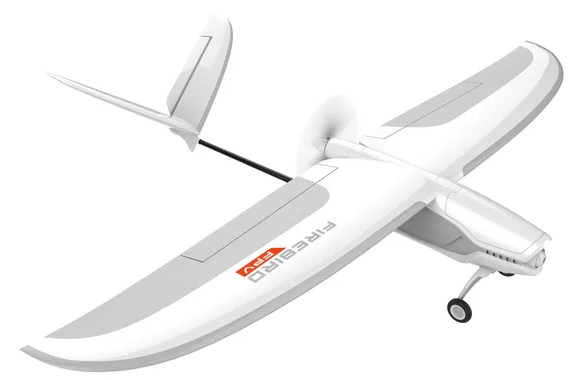
\includegraphics[width=\linewidth]{./img/png/uav-FirebirdFPV-FixedWing.png}
    \caption{Firebird: Fixed-wing~\cite{firebirdDrone}}
    \label{fig:uav-fixed-wing}
  \end{subfigure}\hfill
  \begin{subfigure}[t]{.32\textwidth}\centering
    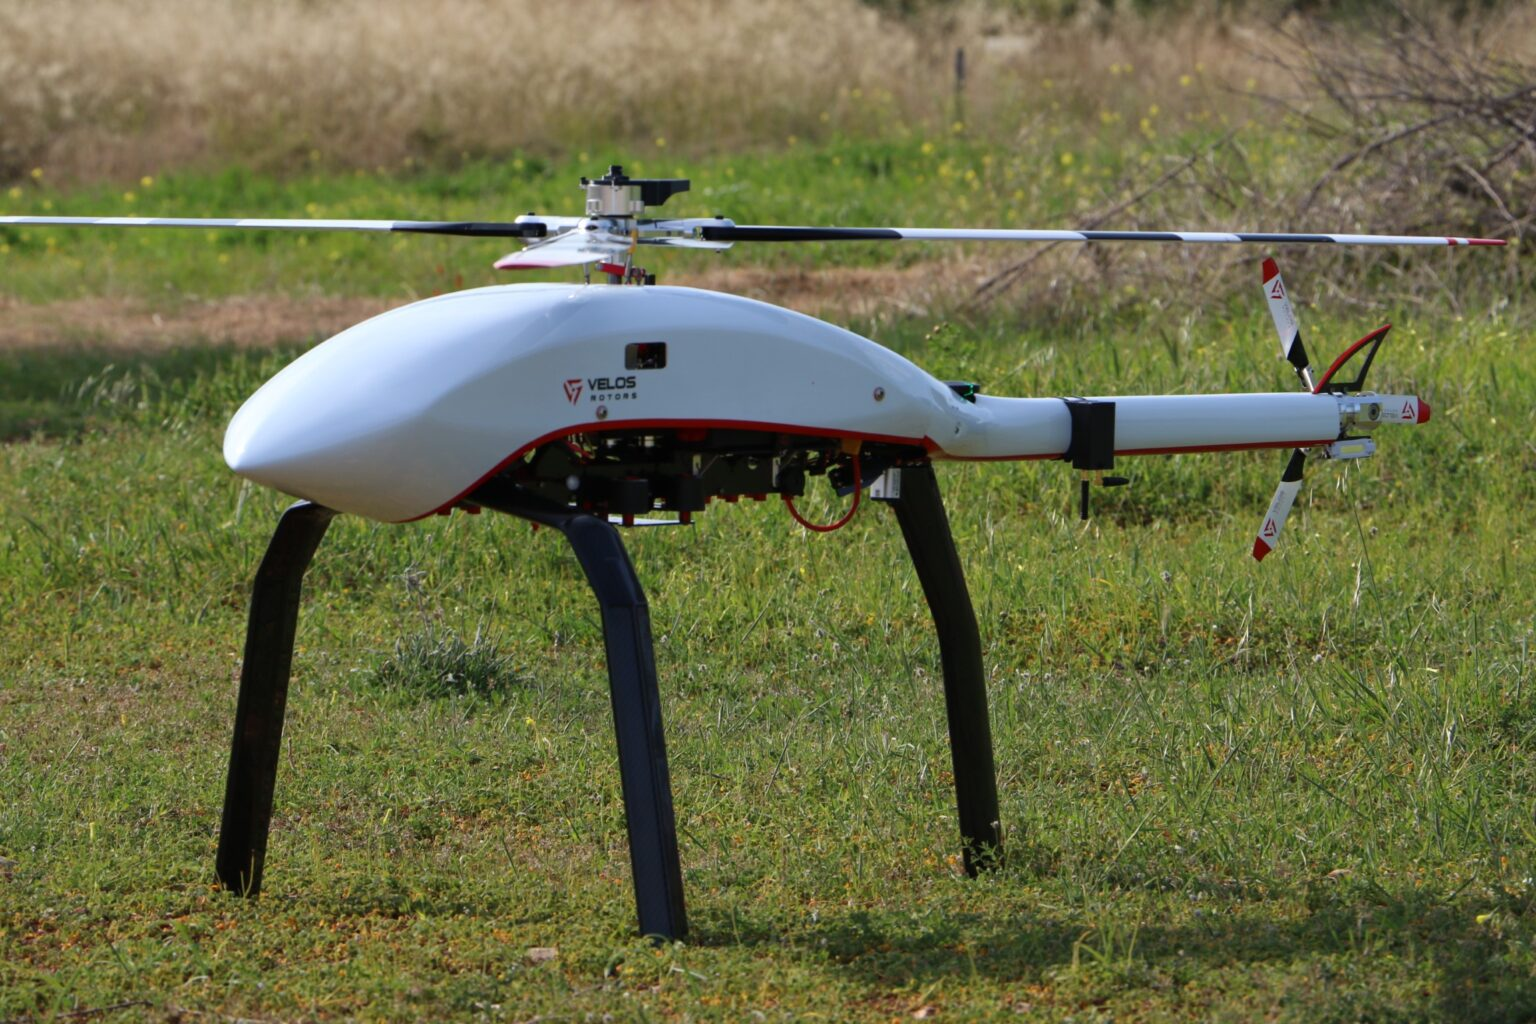
\includegraphics[width=\linewidth]{./img/jpg/uav-velos-singleRotor.jpg}
    \caption{Velos: single-rotor~\cite{velosDrone}}
    \label{fig:uav-single-rotor}
  \end{subfigure}\hfill
  \begin{subfigure}[t]{.32\textwidth}\centering
    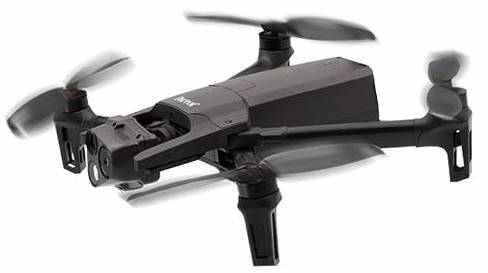
\includegraphics[width=\linewidth]{./img/jpg/uav-parrot-multirotor.jpg}
    \caption{Parrot: multirotor~\cite{parrotDrone}}
    \label{fig:uav-multirotor}
  \end{subfigure}

  \medskip % vertical space between rows

  %--------------------------- Row 2 ---------------------------%
  \begin{subfigure}[t]{.32\textwidth}\centering
    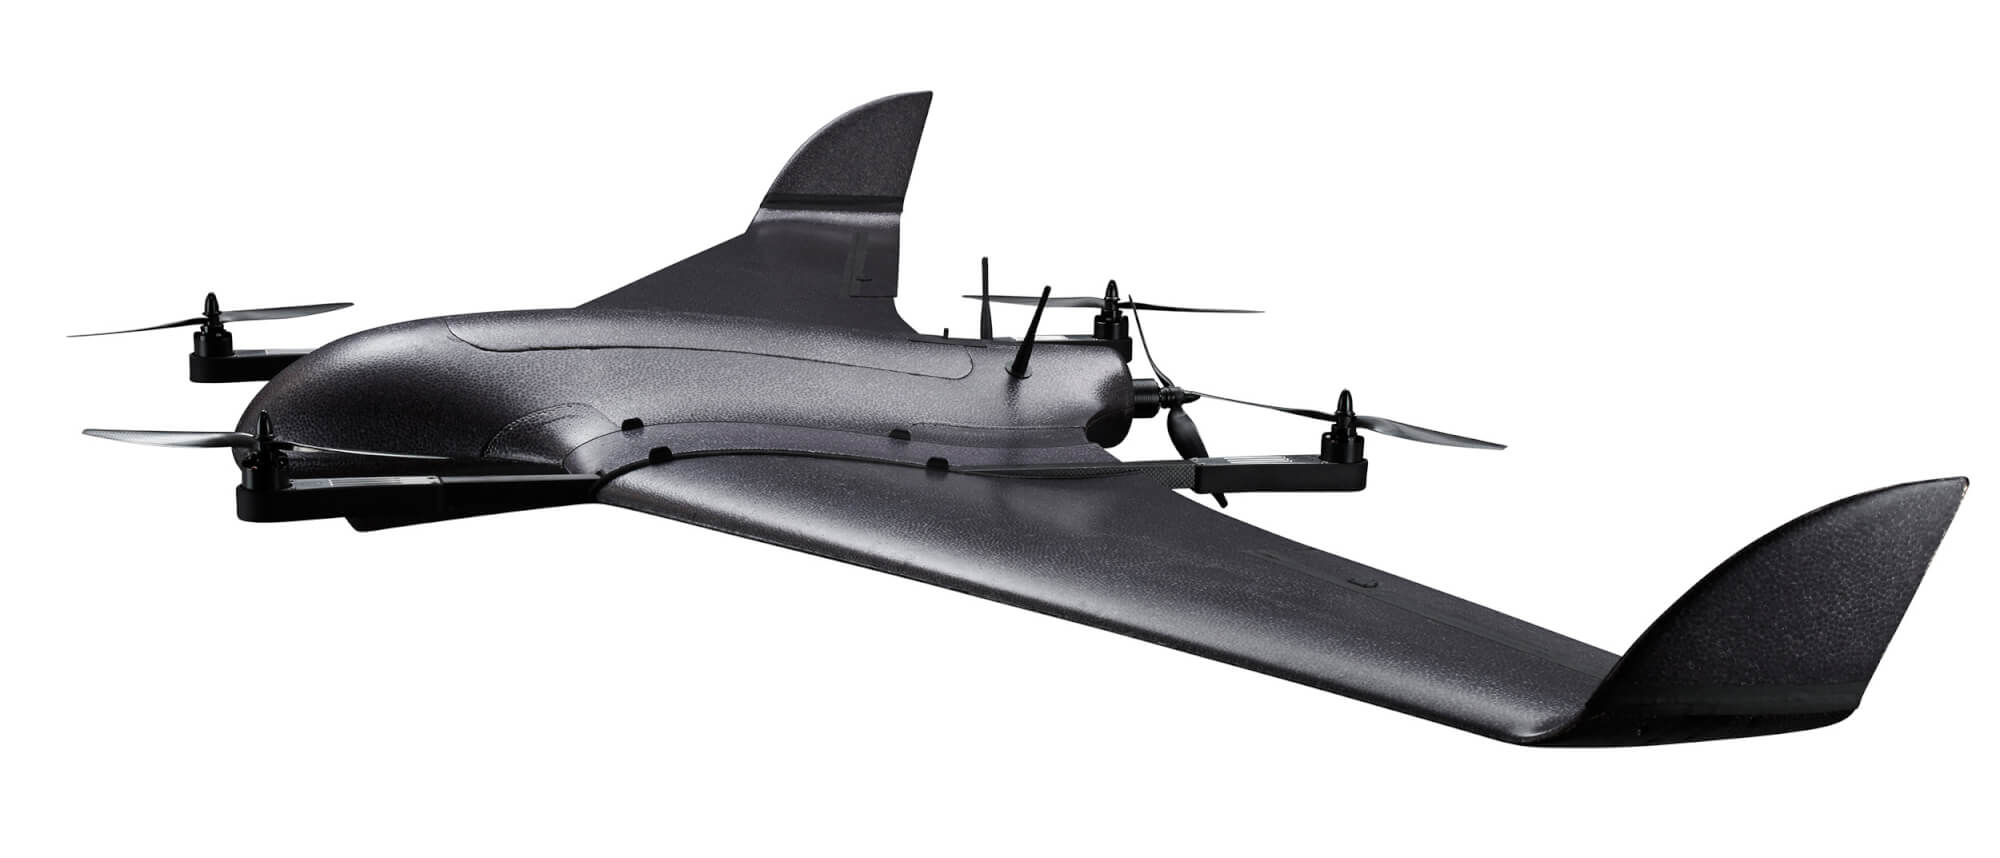
\includegraphics[width=\linewidth]{./img/jpg/uav-deltaQuadPro-hybrid.jpg}
    \caption{DeltaQuad Pro: fixed-wing hybrid~\cite{deltaQuadDrone}}
    \label{fig:uav-fixed-wing-hybrid}
  \end{subfigure}\hfill
  \begin{subfigure}[t]{.32\textwidth}\centering
    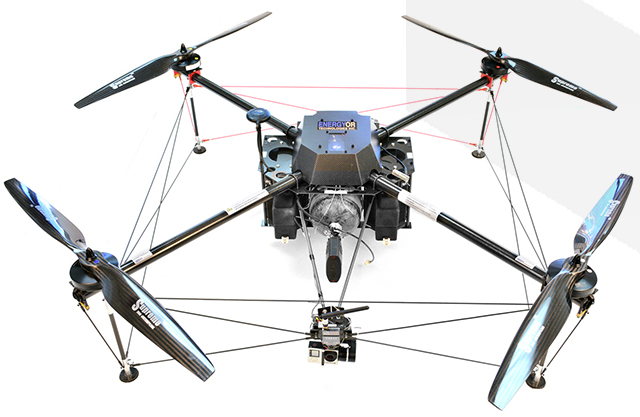
\includegraphics[width=\linewidth]{./img/jpg/uav-energyorQuad1000-hfc.jpg}
    \caption{Energyor Quad 1000: hybrid (HFC + batteries)~\cite{energyorDrone}}
    \label{fig:uav-energyor-hfc}
  \end{subfigure}\hfill
  \begin{subfigure}[t]{.32\textwidth}\centering
    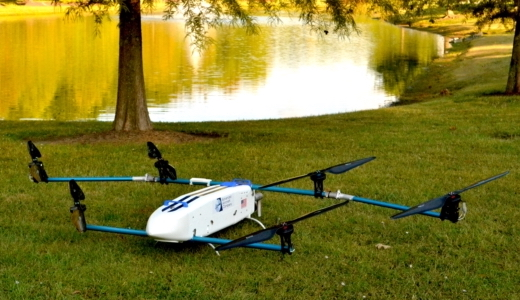
\includegraphics[width=\linewidth]{./img/jpg/uav-HAMR-FuelElectric.jpg}
    \caption{HAMR: hybrid (fuel+batteries)~\cite{hamrDrone}}
    \label{fig:uav-hamr-fuel}
  \end{subfigure}

  \medskip % vertical space between rows

  %--------------------------- Row 3 (centered single) ---------%
  % \makebox centers the single subfigure so the row is "3 x 3 x 1"
  \makebox[\textwidth][c]{%
    \begin{subfigure}[t]{.32\textwidth}\centering
      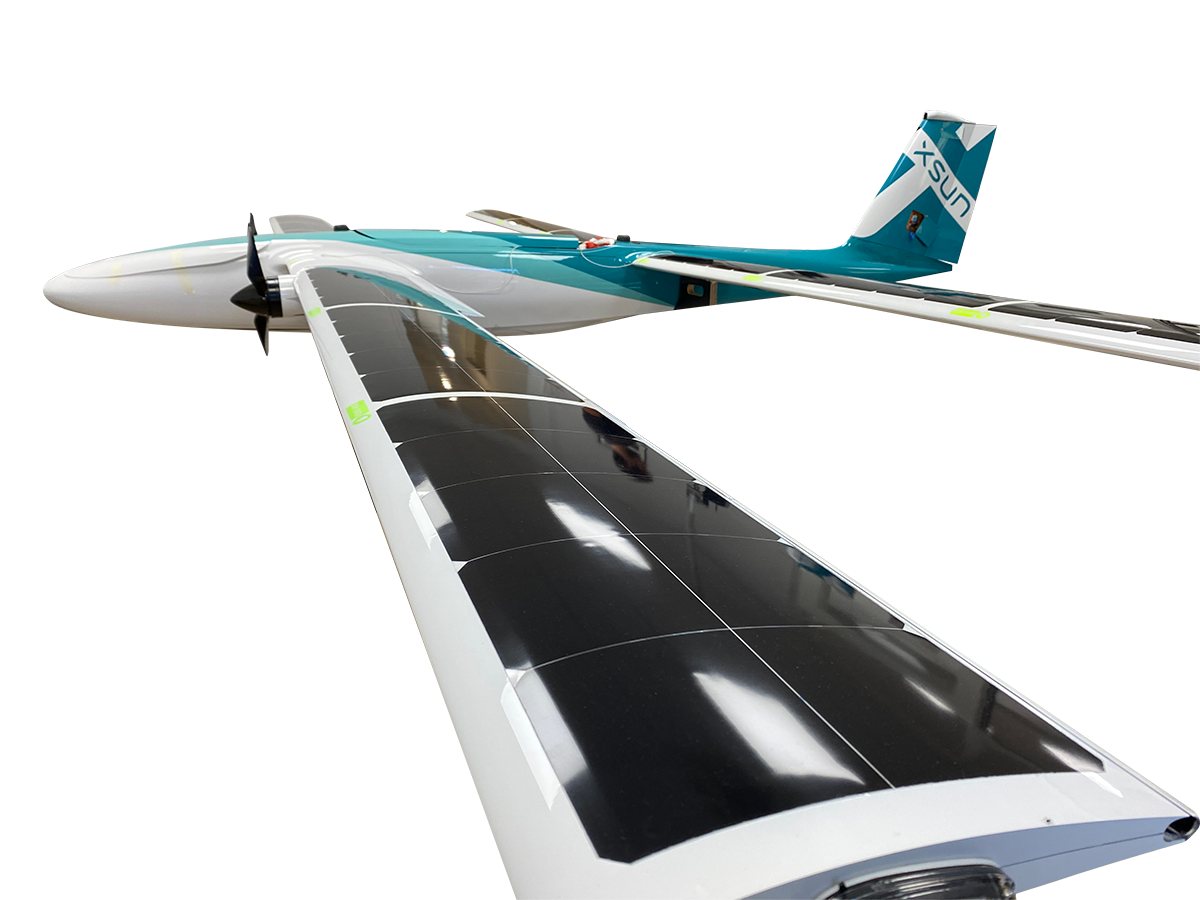
\includegraphics[width=\linewidth]{./img/png/uav-solarXOne.png}
      \caption{Solar X One: solar powered~\cite{solarXOneDrone}}
      \label{fig:uav-solarX}
    \end{subfigure}
  }

  \caption{UAV types examples}
  \label{fig:uav-types}
\end{figure}
%

% Compact UAV classification summary table
\begin{table}[!t]
  \centering
  \caption{UAV classification axes with examples}
  \label{tab:uav-class-summary}
  \begingroup
  \footnotesize
  \setlength{\tabcolsep}{4pt}
  \setlength{\extrarowheight}{0.4ex}
  \renewcommand{\arraystretch}{1.15}
  \begin{tabularx}{\textwidth}{@{}p{2.4cm} p{4.3cm} p{4.3cm} X@{}}
    \toprule
    \textbf{Axis} & \textbf{Categories} & \textbf{Example platforms} & \textbf{Notes} \\
    \midrule
    Flight principles &
      Lighter-than-air; Heavier-than-air (glider, rotorcraft, ornithopter) &
      EBlimp Atom~\cite{eblimp-atom}; PX4 Glider~\cite{px4-glider}; Ornithopter~\cite{drone-bird} &
      Buoyancy vs.\ aerodynamic lift/propulsion. \\
    % \addlinespace[0.2ex]
    Airframe &
      Fixed-wing; Fixed-wing hybrid (VTOL); Single-rotor; Multirotor (tri/quad/hexa/octo) &
      Firebird~\cite{firebirdDrone}; DeltaQuad Pro~\cite{deltaQuadDrone}; Velos~\cite{velosDrone}; Parrot~\cite{parrotDrone} &
      Endurance vs.\ agility trade-offs; hybrids ease runway needs. \\
    % \addlinespace[0.2ex]
    Altitude band &
      \gls{lap} (\(\sim\)3–9\,km); \gls{hap} (\(>\)9\,km) &
      Parrot~\cite{parrotDrone}; Pathfinder Plus~\cite{hale-uas}  &
      \gls{lap} often for comms relays; \gls{hap} for wide-area coverage~\cite{mohsan2022towards}. \\
    % \addlinespace[0.2ex]
    Overall weight &
      Micro (\(<100\)g); Very small (100g–2kg); Small (2–25kg); Medium (25–150kg); Large (\(>150\)kg) &
      BetaFPV Meteor65 Pro~\cite{micro-uav-fpv}; NXP HoverGames~\cite{nxp-hoverGames-uav};
      Hunter10~\cite{medium-uav}; Shadow50~\cite{medium-uav-2}; Reach-S~\cite{large-uav} &
      Example scheme per AU regs~\cite{alladi2022UAVBlockain}; impacts rules and mission profile. \\
    % \addlinespace[0.2ex]
    Power source &
      Battery (LiPo); Fuel (gas/nitro); Hydrogen fuel cell; Hybrid (fuel+bat., HFC+bat.); Solar assist &
      Parrot~\cite{parrotDrone}, DJI Mavic 3~\cite{djiMavic3Drone}; Gas-powered~\cite{gasPoweredDrone}; EnergyOr H2Quad 1000~\cite{energyorDrone}; Flaperon MX8~\cite{flaperonDrone} &
      Energy density vs.\ mass/complexity; hybrids extend endurance at added cost. \\
    % \addlinespace[0.2ex]
    Target audience &
      Recreational/hobby; Commercial/industrial; Defense &
      KK2 flight board~\cite{hobbykingKK2}; Skynode X~\cite{skynodeXWebsite}; Defense-use cases~\cite{vxWorks-uav-northrop,skynodeS-noJamming-2,theDriveUAVAccident2019} &
      Drives cost, openness, certification, and ecosystem. \\
    \addlinespace[0.2ex]
    User modifiability &
      Open/user-modifiable; Proprietary (vendor SDK) &
      Pixhawk4-based (PX4)~\cite{osh-uav}; DJI (SDK)~\cite{djiSDK} &
      Transparency/extensibility vs.\ turnkey integration and market dominance~\cite{droneAnalyst2021}. \\
    \bottomrule
  \end{tabularx}
  \endgroup
\end{table}


\emph{Autonomy/Endurance} is the maximum continuous flight time on a single
energy source (battery, fuel, or hybrid), ranging from \(\sim\)20–30\,min for
small \glspl{uav} to several hours for larger platforms. It is strongly
influenced by size, weight, aerodynamics, and weather.
Ongoing work explores in-flight recharging via renewable sources (\gls{pv}
cells) or wireless power techniques (e.g., lasers emission)~\cite{mohsan2022towards,mohsan_comprehensive_2022}.
\emph{Payload} denotes the lifting capacity, spanning from a few grams (small
\glspl{uav}) to hundreds of kilograms (large \glspl{uav}); common payloads
include sensors and video cameras~\cite{mohsan2022towards}.
\emph{Range} is the maximum command-and-control distance and depends on the
communication technology, network conditions, link budget, and
environment~\cite{mohsan2022towards}.
\emph{Ceiling/Altitude} reflects the maximum operating height, limited by both technological performance (propulsion, energy, airframe) and regulatory constraints~\cite{mohsan2022towards}.
Figure~\ref{fig:uav-mindmap} summarizes these concepts in a generic \gls{uav}
overview.

%
\subsection{System overview}%
\label{sec:system-overview}

Figure~\ref{fig:uav-sysOverv} presents an overview of the \gls{uav} system and its ecosystem with numbered callouts. 
At the core \emph{(1)} are the flight-control hardware and software (flight computer + autopilot), whose main responsibilities include 
path planning, communication management, data acquisition, and mission execution~\cite{aggarwal2020UAVPathPlanning}.

\begin{figure}[!hbt]
  \centering
  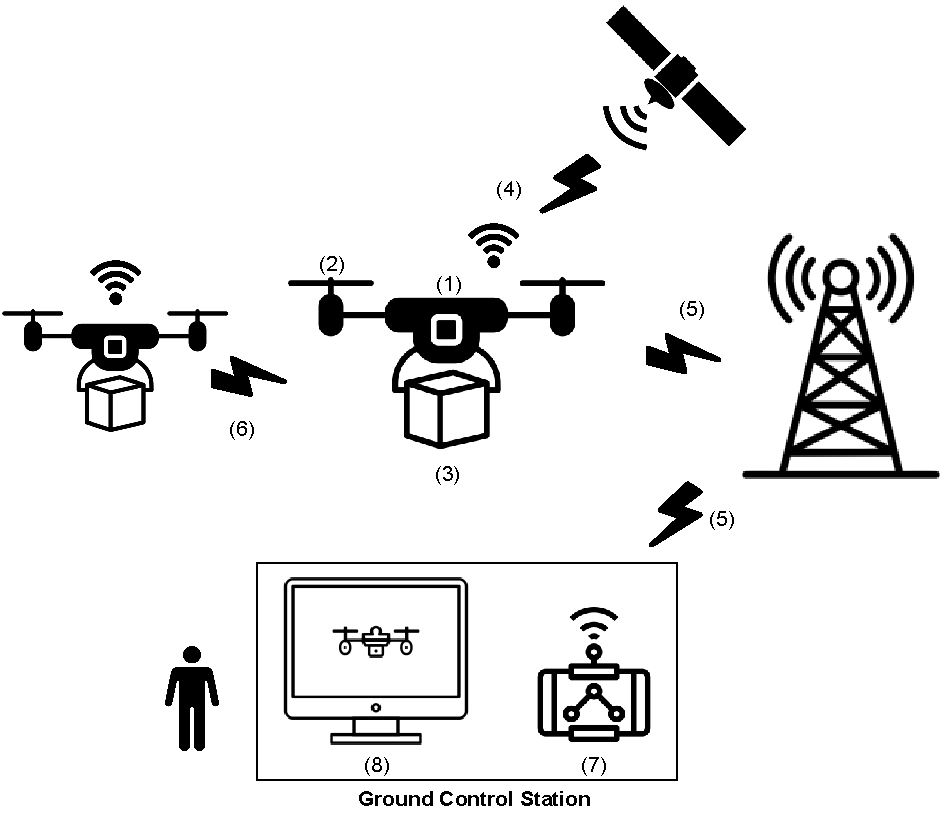
\includegraphics[width=0.7\textwidth]{./img/pdf/uav-sys-overv.pdf}
  \caption[UAV system overview]{UAV system overview (adapted from~\cite{mohsan2022towards,aggarwal2020UAVPathPlanning}).}
  \label{fig:uav-sysOverv}
\end{figure}

% \paragraph{Flight control loop.}
Path planning in \emph{(1)} works together with the ground control station \emph{(5)} to assist navigation, 
find feasible/optimal trajectories, maintain environmental awareness (weather, obstacles), and regulate motion and speed for obstacle avoidance~\cite{aggarwal2020UAVPathPlanning}. 
The on-board flight controller \emph{(1)} fuses data from multiple sensors (e.g., \gls{imu}, barometer, \gls{gps}) with 
commands from the \gls{gcs} \emph{(5)} to perform attitude estimation and control (e.g., Kalman filtering) and to drive the propulsion system \emph{(2)} (motors)~\cite{px4-sysArch}.

% \paragraph{Communications.}
The controller \emph{(1)} typically manages three link classes~\cite{aggarwal2020UAVPathPlanning}: 
(i) \gls{uav}–\gls{gcs} link \emph{(5)}, used for telemetry (including audio/video) and human remote control via the pilot interface \emph{(8)} and handheld/console device \emph{(7)}; 
(ii) \gls{uav}–satellite link \emph{(4)}, which provides weather, climate, and \gls{gps} services for accurate navigation~\cite{liang_toward_2024,alvarez-vanhard_uav_2021}; and 
(iii) \gls{uav}–\gls{uav} inter-vehicle link \emph{(6)}, supporting cooperative missions and shared situational awareness (e.g., hazard signaling)~\cite{li_distributed_2024,azari_uav--uav_2020}.
The mission objective (e.g., video capture, topographic mapping~\cite{caroti_uav-borne_2017}) directly determines the payload \emph{(3)}, such as cameras or \gls{lidar}~\cite{cai_branch_2024}.

% \paragraph{Sensors.}
Sensors on \emph{(1)} are commonly grouped into \emph{obstacle-avoidance}, \emph{payload} \emph{(3)}, and \emph{navigation} classes~\cite{VogeltanzFreeSWUAVSurvey2016}. 
Ultrasonic and infrared sensors are widely used for collision avoidance; \gls{tof} sensors like \gls{lidar} offer better range/precision at higher cost and complexity. 
Navigation typically relies on an \gls{imu} (attitude/heading), a barometer (altitude with centimeter-level precision), and \gls{gnss}/\gls{gps} from \emph{(4)} (global position). 
Because \gls{gps} alone can have errors on the order of meters, fusing \gls{imu} and barometer data is standard to improve accuracy~\cite{ebeidUAVPlatformsSurvey2017}.

% \paragraph{Actuation.}
Electronic propulsion dominates. In multirotors, \glspl{bldc} in the propulsion system \emph{(2)} drive the rotors, controlled by \glspl{esc}—high-frequency inverters that convert \gls{dc} to three-phase \gls{ac} and modulate motor speed~\cite{malyshev_research_2024}. 
Fixed-wing hybrids additionally use servomotors for control surfaces (e.g., flaps)~\cite{gabrielBLDCFixedWingUAV2011}.
Figure~\ref{fig:uav-sysOverv-tasks-mindmap} depicts a concept map of the main tasks and components.
%
% \paragraph{Ecosystem layers.}
The \gls{uav} ecosystem can be outlined as a top-down view of five layers~\cite{glossner2021overview}
(Figure~\ref{fig:uav-sysOverv-hierarc-mindmap}): 
\begin{enumerate}[label=(\arabic*)]
  \item \emph{Flight supervision} (flight management, safety/authorization, remote identification). 
        Commands flow from the \gls{gcs} to the \gls{fcs}; tools such as \lstinline|QGroundControl| provide mission planning, mapping, and live telemetry. 
        Fail-safes (geofencing, low battery, loss of \gls{rc}/datalink) must be enforced by the pilot or autopilot. 
        Airspace authorization can be obtained via \lstinline|LAANC| or \lstinline|Google Wing OpenSky|; since 2023, remote ID mandates broadcasting a unique identifier.

  \item \emph{Command and control}. 
        Ensures safe flight via human or autopilot-generated commands over proprietary links or open \glspl{api} (e.g., MAVLink SDK, Parrot SDK). 
        Notable open-source autopilots include \lstinline|PX4|, \lstinline|ArduPilot|, and \lstinline|Paparazzi UAS|.

  \item \emph{System simulation}. 
        Analyzes behavior under varied conditions via \gls{sitl}/\gls{hitl} (e.g., Gazebo~\cite{garcia_simulation_2022} with PX4~\cite{px4-sim} or ArduPilot~\cite{arduPilot-sim}, CoppeliaSim~\cite{coppelia-sim}) and full flight simulators (FlightGear~\cite{flightgear}).

  \item \emph{Operating systems}. 
        Provide hardware abstraction: open-source \glspl{rtos} (\lstinline|NuttX|~\cite{px4-home}, \lstinline|ChibiOS|~\cite{arduPilot-home}, \lstinline|FreeRTOS|~\cite{librePilot-arch}) and \glspl{gpos} (\lstinline|Linux|~\cite{px4-pilotpi}), as well as proprietary options (\lstinline|VxWorks|~\cite{vxWorks-uav-aribus-helionic}). 
        Some flight stacks also run natively without a full \gls{os} (e.g., \lstinline|Paparazzi UAS|~\cite{paparazzi-github}, \lstinline|INAV|~\cite{inav-github}).

  \item \emph{Physical hardware}. 
        Comprises sensors, compute, communications, and actuators (propulsion and payload), i.e., the electronic platform and effectors that realize the flight and mission functions.
\end{enumerate}


\subsection{Security and Safety}%
\label{sec:security-safety}
Security of the \gls{uav} ecosystem -- and the associated safety of people and
property -- is often underemphasized at design time~\cite{leccadito2018survey}. 
In practice, many platforms ship with onboard wireless links that are open, unencrypted, or unauthenticated, exposing them to a wide range of cyberattacks~\cite{kishnaCyberVulnerUAVReview2017,mansfieldUAVCyberThreats2013}. 
The issue is not confined to consumer systems: in 2017 the U.S.\ Army restricted the use of DJI drones over cybersecurity concerns~\cite{suasNewsDjiDronesBanned2017}. 
Compromise can yield unauthorized control or data exposure, and several media-reported incidents show weaponization risks~\cite{spiegelUAVAccident2015,nytimesUAVAccident2018,theDriveUAVAccident2019}. 
With projected market growth~\cite{mohsan2022towards} and regulations that increasingly permit operations over people~\cite{stocker2017UAVRegulationsReview}, both likelihood and impact of misuse can rise.

Common attacks include \gls{dos} and \gls{ddos}, which degrade availability by
draining batteries, overloading compute, or saturating communication links,
leading to service interruptions~\cite{mohsan2022towards}.
More sophisticated threats span \gls{gps} spoofing (broadcasting counterfeit
satellite signals), \gls{gps} jamming, instrument spoofing (e.g.,
gyroscope/compass), and even killing critical processes~\cite{nassi2021sok}.
Ground control stations are also targeted; keyloggers, malware, and supply-chain
compromises can provide indirect access to the \gls{uav}, enabling data
exfiltration or malicious command injection~\cite{mohsan2022towards}.

Nassi et~al.~\cite{nassi2021sok} provide an extensive survey, classifying
threats by target: the \gls{uav} itself or people.
\emph{Attacks targeting \glspl{uav}} include tampering with onboard electronics
(e.g., counterfeit or unsigned firmware, sensor spoofing, \gls{gps} jamming),
the airframe/payload (e.g., malicious \gls{cad} files, nets, projectiles), the
\gls{gcs} and \gls{fpv} links (e.g., deauthentication, video exfiltration,
remote takeover), and cloud backends used for telemetry.
Mitigations include signed/attested firmware, encrypted/authenticated links with
frequency agility, runtime monitoring and fault
containment~\cite{mohsan2022towards}, parachute systems, and strong access
control (including multi-factor authentication).
\emph{Attacks targeting people} range from privacy violations to kinetic harm against individuals, organizations, or states. 
Counter-\gls{uav} measures follow a detect–assess–interdict pipeline using radar, optical/infrared, \gls{lidar}, and acoustic sensing; each has gaps (e.g., small \gls{uav} radar cross-section, suppressible acoustic signatures)~\cite{sathyamoorthy2015review}. 
Upon confirmation, interdiction options include nets, jammers, birds of prey,
and lasers -- each with distinct effectiveness and safety
trade-offs~\cite{nassi2021sok}.


Safety failures pose risks to people and property and can be grouped into
several categories~\cite{ferrao2020stuart}.
First, \emph{damage from calculation errors} arises when the \gls{uav}'s flight
proves more hazardous than anticipated (e.g., entry into restricted zones).
Second, \emph{sensor failures} occur when onboard sensors miss delicate or
transparent obstacles (wires, branches, glass), leading to collisions, sometimes
compounded by pilot overconfidence.
Third, \emph{obstacle deviation} can cause crashes into buildings or vegetation
due to sudden, unexpected changes in direction.
Fourth, \emph{direct attacks} use \glspl{uav} to harm individuals or steal
payloads (e.g., medical supplies), with recreational or hobbyist platforms
frequent targets.
Finally, \emph{accidental damage} results when a \gls{uav} goes out of control
due to operator error, cyberattack, or software/hardware malfunction.
Regardless of cause, a falling aircraft can inflict severe harm on people and
goods.

Security and safety are fundamental to \gls{uav} operation, yet reducing attack
vectors and overall attack surface requires deliberate design choices.
Ferrão~\cite{ferrao2020stuart} argues that \gls{uav} design should address both dimensions simultaneously, as they strongly influence each other. 
Figure~\ref{fig:uav-security-mindmap} illustrates the \gls{uav} security and safety taxonomy.

\subsection{UAV Reference Hardware}%
\label{sec:uav-ref-hw}
In this section we discuss reference hardware for \glspl{uav}. 
We first present an overview of the hardware architecture, then analyze open-source and commercial solutions in more depth.

\subsubsection{Overview and Architecture}%
\label{sec:overv-arch-hw}
Figure~\ref{fig:uav-hw-arch} illustrates a high-level abstraction of the \gls{uav} hardware architecture~\cite{leccadito2018survey,px4-sysArch}. 
The main computing platforms are shown in orange: (1) the flight controller or \gls{fmu} (e.g., Pixhawk) and (2) an optional companion computer that offloads the \gls{fcs}. 
The companion can assist with navigation (collision avoidance), support mission tasks (e.g., camera surveillance, topographic mapping), and process telemetry data.

\begin{figure}[!hbt]
  \centering
  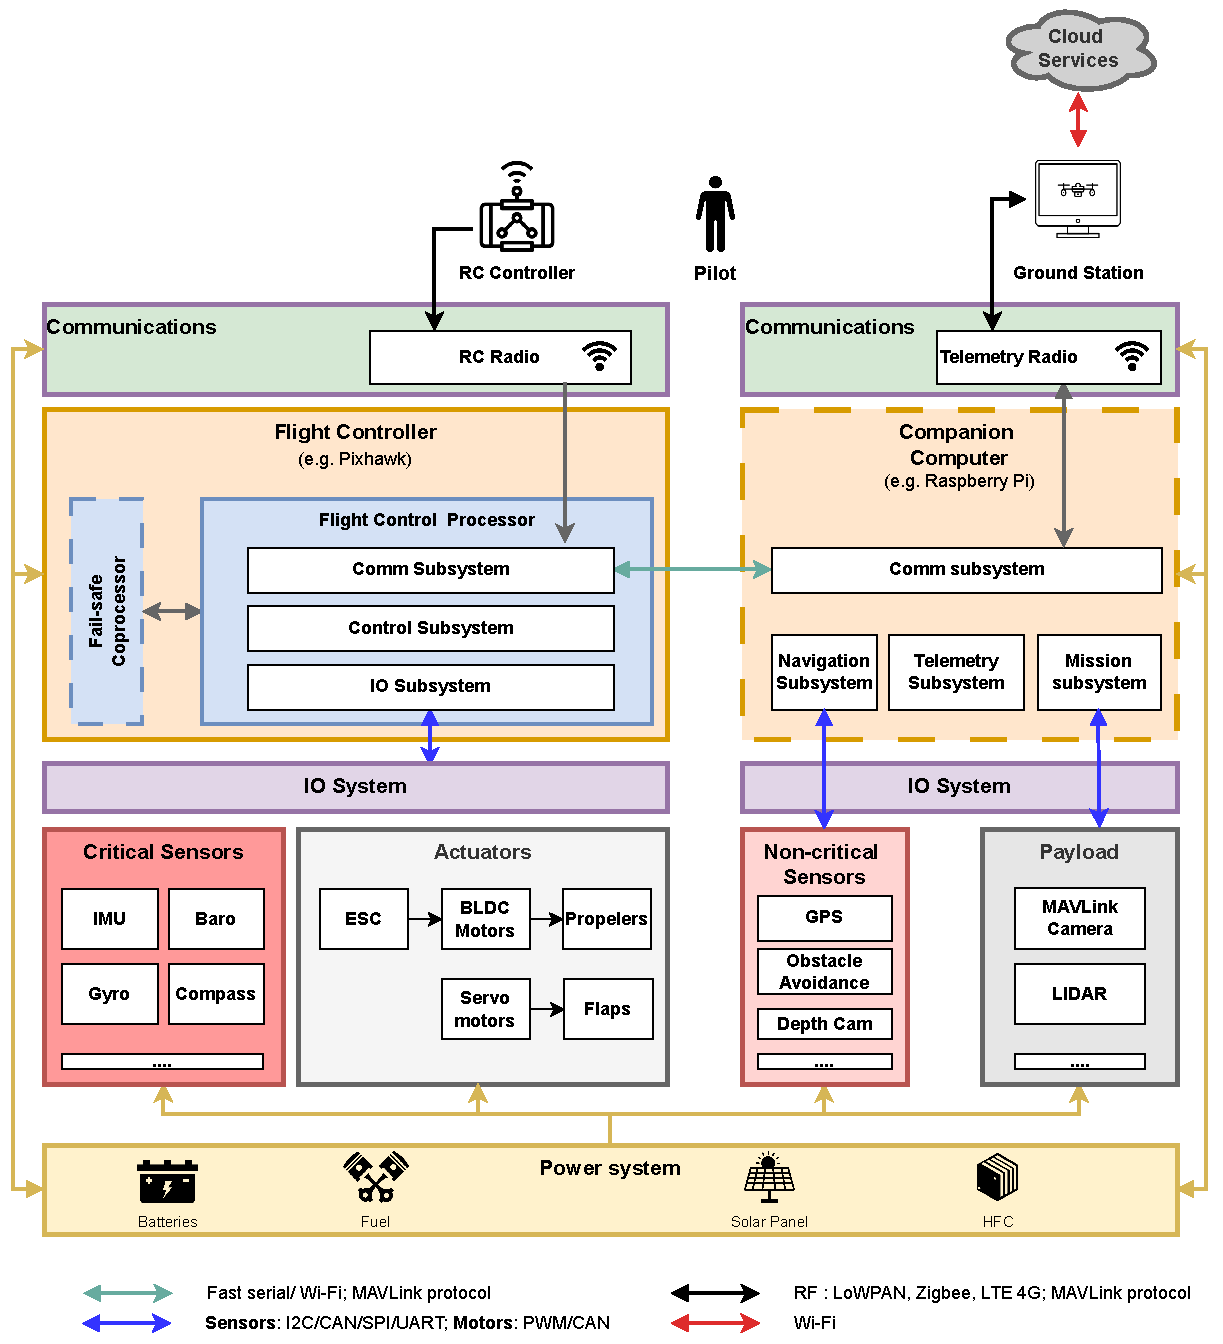
\includegraphics[width=\textwidth]{./img/pdf/uav-hw-arch.pdf}
  \caption{UAV hardware architecture: high-level abstraction.}
  \label{fig:uav-hw-arch}
\end{figure}

The \gls{fcs} typically comprises a main processor for \gls{uav} control and, optionally, a fail-safe coprocessor dedicated to handling contingencies (e.g., return-to-home on low battery). 
The main processor handles: (i) communications, processing commands from the manual \gls{rc} controller and from the companion computer; 
(ii) aircraft control, typically using \gls{pid} and estimation methods (e.g., Kalman filtering); and 
(iii) \gls{io}, interfacing critical sensors (e.g., \gls{imu}, barometer, gyroscope, compass) and actuators (e.g., \glspl{bldc}, servomotors). 
The power system supplies energy to computation and \gls{io}.

While the flight controller does not require a companion computer for line-of-sight manual flight, autonomous missions typically depend on non-critical sensors such as \gls{gps} and obstacle-avoidance sensors. 
In this mode, the companion computer transmits telemetry to the \gls{gcs} -- often
overlaid on a map for navigation -- and receives navigation and mission commands,
processing them and dispatching lower-level commands to the flight controller or
\gls{io} subsystem.

\subsubsection{Open-source solutions}%
\label{sec:open-source-solut-hw}

\glsxtrfull{osh} platforms aim for transparency, extensibility, flexibility, and maintainability while remaining cost-effective. 
By \gls{osh} we mean that the hardware design (mechanical drawings, schematics, \gls{bom}, \gls{pcb} layout data, \gls{hdl} sources) and the software that drives the hardware are released under free/libre terms~\cite{freeGNU}. 
Users can purchase or manufacture components individually or acquire \gls{cots} kits.

Historically, \gls{osh} solutions fall into three broad families~\cite{ebeidUAVPlatformsSurvey2017}: Atmel-based, Arm-based, and companion-computer-based platforms. 
The first two target the \gls{fmu}; the last co-packages an \gls{fmu} and a companion computer.

\paragraph{Atmel-based (legacy).}
Until recently, 8-bit Atmel platforms such as the ArduPilot Mega (APM) were still in production. 
APM is built around the ATmega2560 \gls{mcu}, typically paired with an \gls{imu} and, optionally, a compass and \gls{gps}~\cite{ardupilotMega}. 
A key advantage was Arduino \gls{ide} compatibility, which enabled hobbyists to customize ArduPilot features easily. 
However, the complexity of modern autopilots requires more capable 32-bit \glspl{mcu}, leading to the deprecation of many 8-bit designs~\cite{fmu8BitDeprecation}.

\paragraph{Arm-based flight controllers.}
The vast majority of current \gls{osh} projects use 32-bit Arm \glspl{mcu} 
(\lstinline|Pixhawk 4|, \lstinline|CC3D|, \lstinline|Paparazzi Chimera|, \lstinline|CUAV v5 Plus|, etc.), supported by open hardware specifications such as the Pixhawk standards~\cite{pixhawk}. 
The \lstinline|Pixhawk 4| (Figure~\ref{fig:osh-pixhawk4}) was developed by Holybro in collaboration with the PX4 team for academic and commercial use~\cite{pixhawk4}. 
It is released under a \gls{bsd} license and integrates two 32-bit Arm processors: a Cortex-M7 STM32F765 as the \gls{fmu} and a Cortex-M3 STM32F100 as the \gls{io} coprocessor. 
Pixhawk 4 provides on-board sensors (accelerometers/gyroscopes, magnetometer, barometer) and a \gls{gps} module, and exposes standard interfaces (\gls{pwm}, \gls{can}, \gls{i2c}, \gls{uart}, \gls{spi}) for sensors and actuators. 
\gls{uart} and telemetry ports also support off-board computers~\cite{pixhawk4} and remote controllers. 
The board typically runs PX4 atop the NuttX \gls{rtos}.

The \lstinline|CUAV v5 Plus| is another open controller that uses a dual-Cortex-M7 architecture for \gls{fmu} and \gls{io}, released under a \gls{bsd} license and commonly running ArduPilot~\cite{arduPilot-cuavV5}. 
In contrast, the \lstinline|Paparazzi Chimera| integrates \gls{io} on a single board around a Cortex-M7 STM32F767 \gls{mcu}, is released under the \gls{gpl}, and runs the Paparazzi autopilot~\cite{paparazziChimera,paparazzi-github}. 
These Arm-based boards typically feature up to \(\sim\)2\,MiB of Flash and \(\sim\)512\,KiB of \gls{sram}.

% Pixhawk 4
\begin{figure}[!hbt]
  \centering
  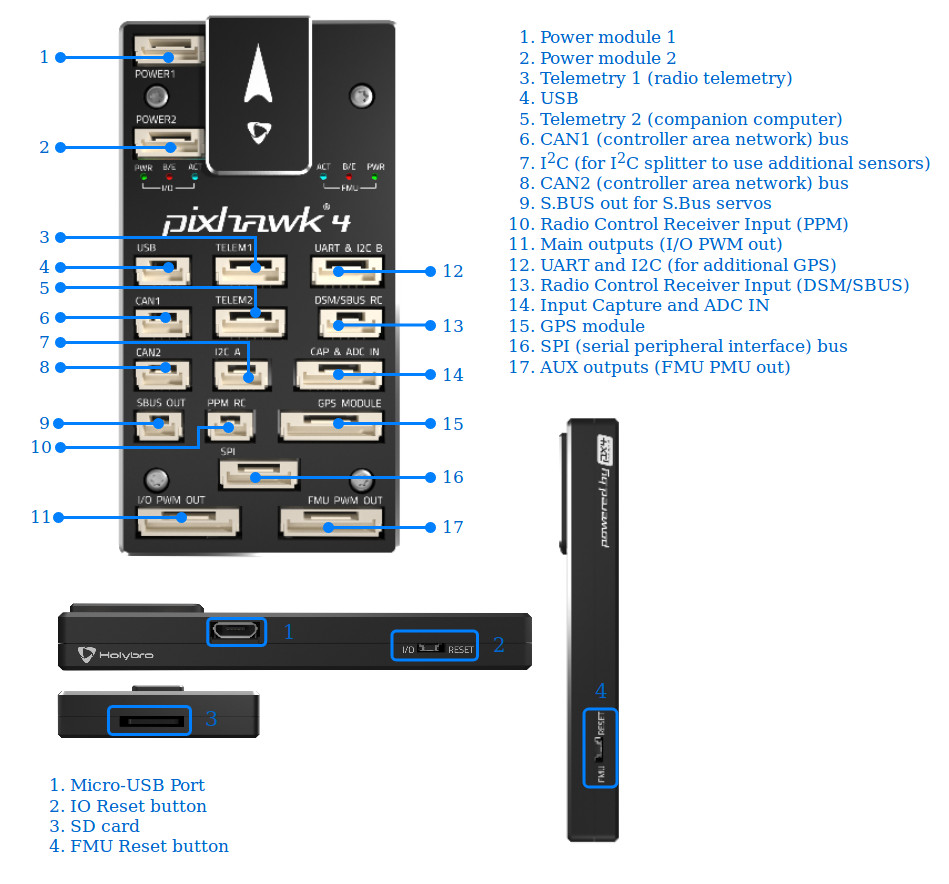
\includegraphics[width=0.7\textwidth]{./img/jpg/osh-pixhawk4.jpg}
  \caption[Pixhawk 4 flight controller]{Pixhawk 4 flight controller~\cite{pixhawk4}\footnotemark}
  \label{fig:osh-pixhawk4}
\end{figure}
\fnlicCCFour{foot:cc-lic-pix}% CC licence

\paragraph{Companion-computer-based stacks.}
These platforms expand \gls{io} via a daughterboard and run the flight stack on an Arm Cortex-A companion under a Linux \gls{gpos} (often with PREEMPT or PREEMPT\_RT), e.g., Erle-Brain 3 and PXFmini~\cite{ebeidUAVPlatformsSurvey2017,erle-brain}. 
PXFmini, designed for the Raspberry Pi Zero, weighs about 15 grams and adds an on-board barometer and \gls{imu}, expansion ports, and triple-redundant power~\cite{pxfmini}. 
Both Erle-Brain 3 and PXFmini have since been deprecated~\cite{pxfmini-deprec}.

\paragraph{Raspberry Pi shields.}
The \emph{PilotPi} shield targets hobbyists by enabling PX4 to run directly on Raspberry Pi with no proprietary drivers and fully open \gls{pcb} designs and schematics~\cite{px4-pilotpi}. 
Figure~\ref{fig:pilotpi} shows the shield stacked on a Raspberry Pi 4. 
The intermediate board integrates typical \gls{uav} sensors (\gls{imu}, compass, barometer) and exposes \gls{gps} and telemetry radios as \gls{uart} devices. 
The top board handles power distribution/management, motor actuation, and peripherals via the \gls{gpio} header.

\begin{figure}[!hbt]
  \centering
  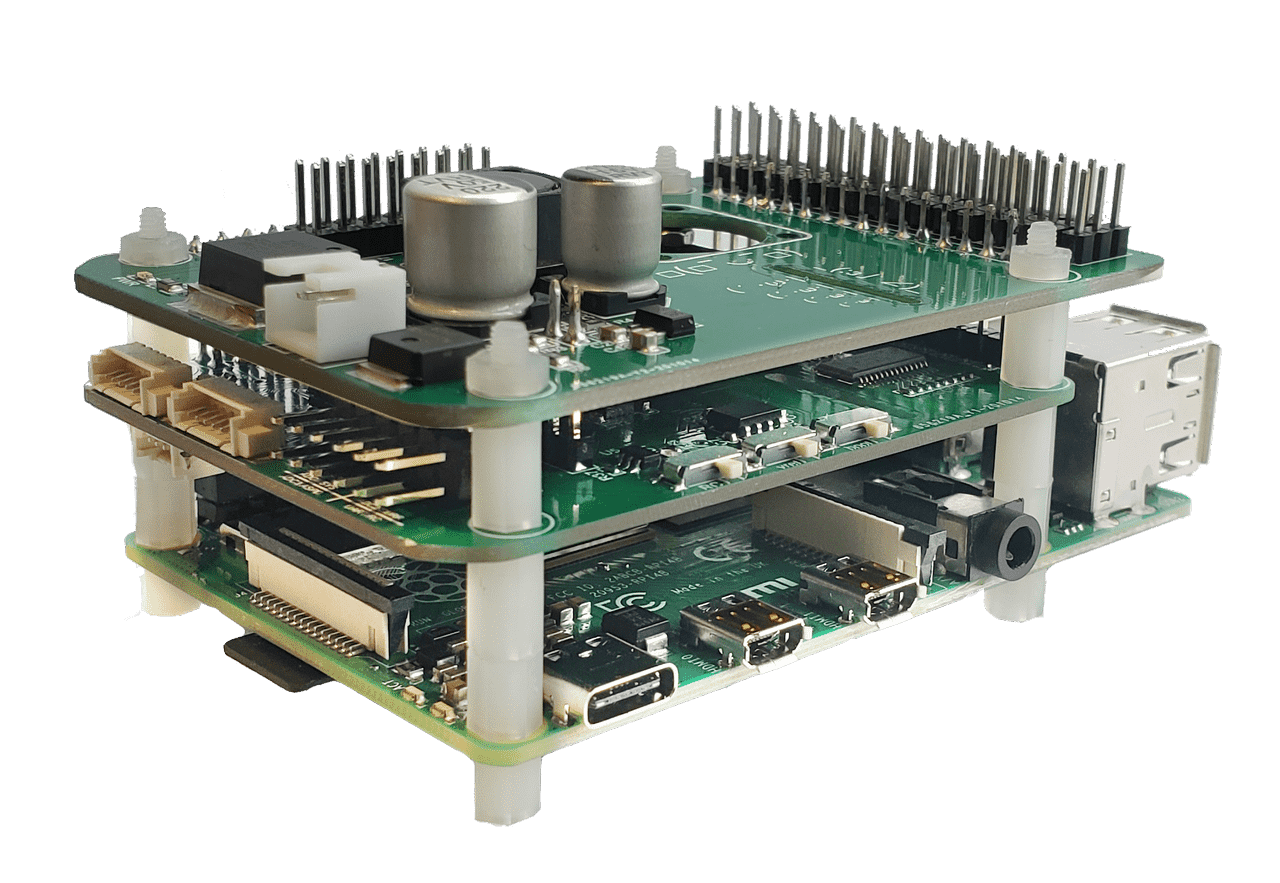
\includegraphics[width=0.7\textwidth]{./img/png/rpi-pilotpi}
  \caption[PilotPi shield]{PilotPi shield~\cite{px4-pilotpi}\footnotemark}
  \label{fig:pilotpi}
\end{figure}
\fnlicCCFour{foot:cc-lic-pilotpi}% CC licence

\subsubsection{Commercial solutions}%
\label{sec:commercial-solutions-hw}
Commercial platforms are generally proprietary and thus closed source. 
This lack of transparency can raise concerns, as illustrated by the U.S.\ Army’s restrictions on DJI drones over cybersecurity issues~\cite{suasNewsDjiDronesBanned2017,djiBan2022}. 
Nevertheless, proprietary solutions account for a large share of the market, with DJI the dominant manufacturer~\cite{droneAnalyst2021}.

Commercial offerings can be grouped into three categories: microcontroller-based, \gls{fpga}-based, and companion-computer-based platforms. 
Historically, 8-bit Atmel designs such as the HobbyKing KK2.1.5 are noteworthy. 
This board used an ATmega644PA 8-bit AVR (64\,KB Flash) to run the KK2 firmware, an MPU-6050 \gls{imu}, and included an \gls{lcd} with push buttons for user interaction~\cite{hobbykingKK2}. 

\paragraph{Microcontroller-based.}
The \lstinline|SPRacing H7 Extreme| is a performance-oriented flight controller built around an Arm STM32H750 \gls{mcu}~\cite{spRacing}. 
It includes external 128\,MB Flash and common onboard sensors and interfaces. 
Targeted at the racing market, it supports \gls{fpv} video via camera inputs~\cite{spRacing} and typically runs \lstinline|Betaflight| or \lstinline|Cleanflight|, though it is also compatible with \lstinline|ArduPilot|~\cite{arduPilot-SPRacing}.

\paragraph{FPGA\,+\,SoC platforms.}
The \lstinline|Aerotenna OcPoC-Zynq Mini| combines an Artix-7 \gls{fpga} with a dual-core Arm Cortex-A9 \gls{soc} and supports PX4 and ArduPilot~\cite{ocpoc} (Figure~\ref{fig:hw-ocpoc}). 
Released in 2017 and now discontinued~\cite{ocpoc-discontinued}, it offered \gls{fpga}-based flexibility for I/O customization and acceleration (including \gls{ai} use cases), while Linux on the Cortex-A9 handled autopilot hosting, logging, and processing. 
It featured 512\,MB \gls{ram}, 128\,MB Flash, and supported triple redundancy for \gls{gps}, magnetometers, and \glspl{imu} in addition to conventional sensors~\cite{ocpoc}.

\begin{figure}[!hbt]
  \centering
  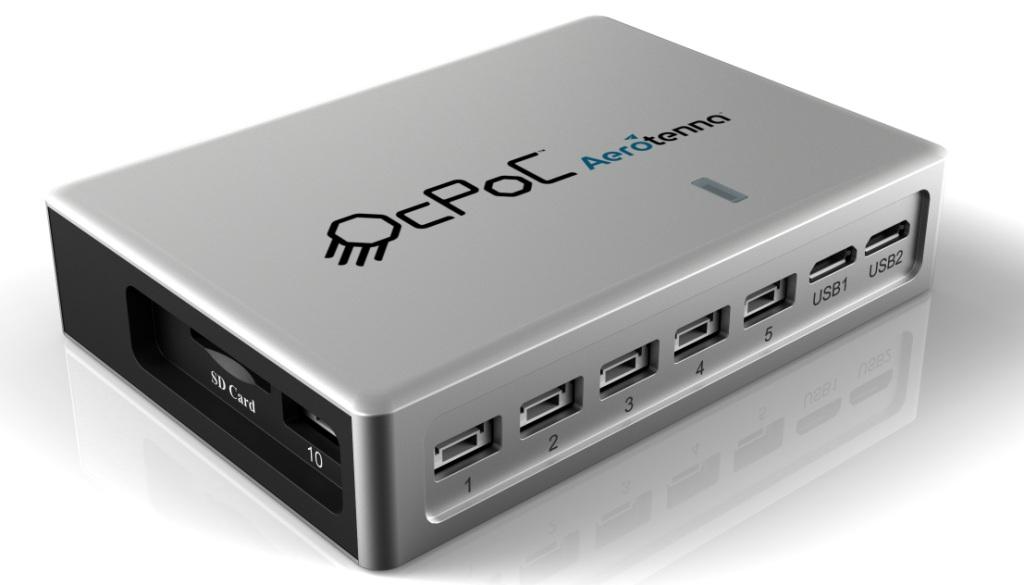
\includegraphics[width=0.5\textwidth]{./img/png/hw-ocpoc-zynq-mini.png}
  \caption[Aerotenna OcPoC-Zynq Mini flight controller]{Aerotenna OcPoC-Zynq Mini flight controller~\cite{ocpoc}\footnotemark}
  \label{fig:hw-ocpoc}
\end{figure}
\fnlicCCFour{foot:ocpoc}%

\paragraph{Companion-computer-based.}
Representative examples include \lstinline|Navio2|, \lstinline|PixC4-Jetson|, and \lstinline|Auterion Skynode X/S|.
Like PilotPi, \lstinline|Navio2| is a Raspberry Pi shield, but its hardware design is closed source. 
It runs a customized Raspberry Pi OS (Debian-based)~\cite{navio2-sw} and supports both ArduPilot and PX4~\cite{arduPilot-Navio2,navio2-px4}. 
The shield integrates dual \gls{imu}, a barometer, a \gls{gnss} receiver, an \gls{rc} I/O coprocessor, \gls{i2c} and \gls{uart} for sensors and radios, 14 \gls{pwm} servo outputs, and triple-redundant power~\cite{arduPilot-Navio2}.

The \lstinline|PixC4-Jetson| (Figure~\ref{fig:hw-horizonJetson}) is a professional controller that pairs dual-Arm \gls{fmu}/I/O processors with an NVIDIA Jetson companion~\cite{arduPilot-horizonJetson}. 
It supports PX4 and ArduPilot and can be configured remotely via terminal access~\cite{arduPilot-horizonJetson}, which necessitates additional security hardening. 
To this end, it provides \gls{lte} connection management with a Layer-2 peer-to-peer \gls{vpn} and a secure cloud backend~\cite{arduPilot-horizonJetson}. 
Live video is supported through multi-endpoint encoding pipelines and an optional low-latency WebRTC distribution service. 
The Jetson companion is well suited to computer vision, machine learning, and \gls{ai} workloads~\cite{jetson-docs}.

\begin{figure}[htb!]
  \centering
  \begin{subfigure}[t]{0.9\textwidth}
    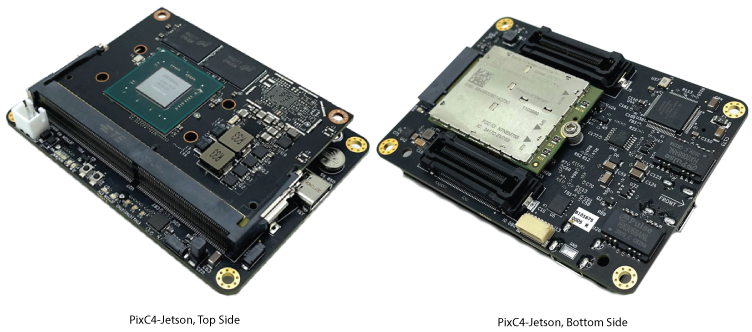
\includegraphics[width=1.0\textwidth]{./img/png/hw-horizon-pixc4-jetson.png}
    \caption{Board}
    \label{fig:hw-horizonJetson-board}
  \end{subfigure}

  \begin{subfigure}[t]{0.9\textwidth}
    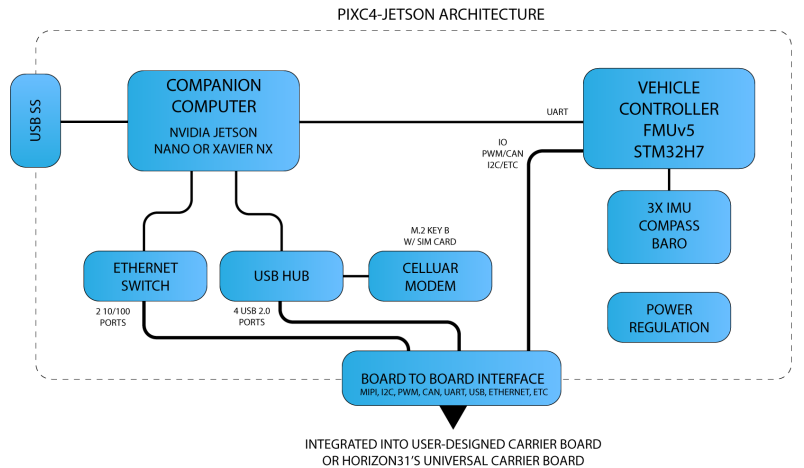
\includegraphics[width=1.0\textwidth]{./img/png/hw-horizon-pixc4-jetson-arch.png}
    \caption{HW architecture}
    \label{fig:hw-horizonJetson-arch}
  \end{subfigure}

  \caption[Horizon31 PixC4-Jetson flight controller]{Horizon31 PixC4-Jetson flight controller~\cite{arduPilot-horizonJetson}\footnotemark}
  \label{fig:hw-horizonJetson}
\end{figure}
\fnlicCCFour{foot:jetson-hw-sw}%

Another notable option is \lstinline|Auterion Skynode X|, which integrates a
flight controller, a mission computer, and LTE connectivity in a compact form
factor~\cite{skynodeXWebsite}.
The \gls{fmu}, based on Pixhawk FMUv6, uses an STM32H753 microcontroller and an STM32F103 I/O coprocessor, with triple-redundant inertial sensing to reduce failure risk~\cite{skynodeXDatasheet}. 
It provides up to 8 \gls{uart}, dual-redundant \gls{can}, 100Base-TX Ethernet, 16 \gls{pwm} outputs, 2 \gls{i2c}, and 1 \gls{spi} interface. 
The \gls{fmu} runs an enterprise-hardened PX4 variant (APX4)~\cite{skynodeXDatasheet}. 
The mission computer features a quad-core Arm Cortex-A53 at 1.8\,GHz, embedded GPUs (GCNanoUltra for 3D and GC320 for 2D), 4\,GB \gls{ram}, and 16\,GB \gls{emmc} + 128\,GB internal \gls{sd} storage~\cite{skynodeXDatasheet}. 
Connectivity includes Wi-Fi, Bluetooth 5, and an LTE module; only USB 2.0 is exposed, as USB 3.0 may interfere with \gls{gps}~\cite{skynodeXDatasheet}. 
Auterion OS (Linux based) communicates with the autopilot via the Auterion SDK~\cite{skynodeX-px4}. 
Supported vehicle types include multicopter, \gls{vtol} airplane, and airplane, reportedly up to 500\,kg takeoff weight; the price is around USD~1900~\cite{skynodePrice}.

Announced in June 2024, \lstinline|Auterion Skynode S| is a compact, lower-cost
variant integrating \gls{fmu} and mission computer in a 49\,mm \(\times\) 37\,mm
footprint~\cite{skynodeS-pressRelease}.
It features an FMUv6x \gls{fmu} and a mission computer with a dedicated
2.3\,\gls{tops} \gls{npu} for \gls{ai} and computer-vision
applications~\cite{skynodeS-pressRelease}.
Its \gls{ai} capabilities have enabled autonomous target tracking, including
moving targets, reported to be resilient to \gls{gps} jamming or
denial~\cite{skynodeS-noJamming}.
Operational reports claim a rise in mission success probability from 20\% to
90\% in the presence of electronic warfare~\cite{skynodeS-noJamming-2}.
%
Table~\ref{tab:hw-ref} summarizes the \gls{uav} reference hardware.
      % >{\raggedright\arraybackslash}p{1.5cm}  % Platform
      % >{\raggedright\arraybackslash}p{1.2cm}  % Type
      % >{\raggedright\arraybackslash}X         % Notes (flex)
      % >{\raggedright\arraybackslash}p{2.1cm}  % Software
      % >{\raggedright\arraybackslash}p{2.4cm}  % Sensors
      % >{\raggedright\arraybackslash}p{2.4cm}  % Interfaces
      % >{\raggedright\arraybackslash}p{1cm}  % Specs.
      % >{\raggedright\arraybackslash}p{1cm}  % Refs.
\begin{table}[!htbp]
  \centering
  \caption{UAV hardware reference summary}
  \label{tab:hw-ref}

  %---- Local settings (this table only) ----
  \begingroup
    \setlength{\tabcolsep}{3.5pt}   % tighter columns (default ~6pt)
    \renewcommand{\arraystretch}{1.05}
    \scriptsize                    % use \footnotesize if you prefer

    % 7 columns total: 6 fixed p{..} widths you can edit, 1 flexible X for Notes
    % Order: Platform, Type, Specs., Software, Sensors, Interfaces, Notes
    \begin{tabularx}{\textwidth}{@{}
      >{\raggedright\arraybackslash}p{2.2cm}  % Platform
      >{\raggedright\arraybackslash}p{1.2cm}  % Type
      >{\raggedright\arraybackslash}X  % Specs.
      >{\raggedright\arraybackslash}p{2.1cm}  % Software
      >{\raggedright\arraybackslash}p{2.4cm}  % Sensors
      >{\raggedright\arraybackslash}p{2.4cm}  % Interfaces
      >{\raggedright\arraybackslash}p{1cm}         % Notes (flex)
    @{}}
      \toprule
      \textbf{Platform} & \textbf{Type} & \textbf{Specifications} & \textbf{Software} &
      \textbf{Sensors} & \textbf{Interfaces} & \textbf{Notes} \\
      \midrule

      APM 2.8 & OSH & FMU: ATMega 2560 & ArduPilot & IMU; Magnetometer; Barometer & UART; I2C & D \\
      Pixhawk 4 & OSH & FMU: STM32F765; IO Processor: STM32F100 & PX4 & IMU; Magnetometer; Barometer; GPS & SPI; I2C; CAN; UART & \mbox{~} \\
      CC3D Revo & OSH & FMU: STM32F405RGT6 & LibrePilot; ArduPilot & IMU; Magnetometer; Barometer & SPI; I2C; UART; CAN; USB; RF Modem & D \\
      Paparazzi Chimera & OSH & FMU: STM32F767 & Paparazzi UAS & IMU; Barometer & SPI; I2C; CAN; UART; XBEE; USB & \mbox{~} \\
      CUAV v5 Plus & OSH & FMU: STM32F765 & PX4 & IMU; Magnetometer; Barometer & SPI; I2C; CAN; UART & \mbox{~} \\
      Erle-Brain 2 & OSH & FMU + CC: Raspberry Pi 3 & Linux + ArduPilot; PX4 & IMU; Magnetometer; Barometer; temperature & SPI; I2C; UART; USB; Ethernet; Bluetooth & D \\
      PXFMini & OSH & FMU + CC: Raspberry Pi Zero & Linux + PX4 & IMU; Magnetometer; Barometer & I2C; UART & D \\
      PilotPi & OSH & FMU + CC: Raspberry Pi 2/3/4 & Linux + PX4 & IMU; Magnetometer; Barometer & SPI; I2C; UART; USB; Ethernet; Bluetooth; Wi-Fi; CSI & E \\
      HobbyKing KK2 & C & FMU: ATMega 644PA & KK2 & IMU; Magnetometer; Barometer & \mbox{~} & D \\
      SPRacing H7 Extreme & C & FMU: STM32H750 & PX4; Betaflight; Cleanflight & IMU; Barometer & SPI; I2C; UART; IR; USB & \mbox{~} \\
      Aerotenna OcPoc-Zynq Mini & C & FMU + CC: Dual-Core Arm A9; IO: Artix-7 FPGA with 28K logic cells & Linux + PX4 & IMU; Barometer & SPI; I2C; UART; USB; CSI; CAN & D \\
      Navio2 & C & FMU + CC: Raspberry Pi 3; RC I/O coprocessor & Linux + PX4; ArduPilot & IMU; Barometer & SPI; I2C; UART; USB; GNSS & \mbox{~} \\
      PixC4-Jetson & C & FMU: STM32H743; IO Processor: STM32F103; CC: Nvidia Jetson & ArduPilot; PX4 & IMU; Magnetometer; Barometer & SPI; I2C; UART; CAN; USB; Ethernet & \mbox{~} \\
      Auterion Skynode X & C & FMU: STM32H753; IO Processor: STM32F103; CC: Quad-core Arm Cortex-A53 & APX4 & IMU; Magnetometer; Barometer & SPI; I2C; UART; CAN; Ethernet; Wi-Fi; Bluetooth; LTE module & \mbox{~} \\
      Auterion Skynode S & C & FMU: Arm Cortex-M7; CC: Quad-core Arm Cortex-A53; NPU: 2.3 TOPS & APX4 & IMU; Magnetometer; Barometer & SPI; I2C; UART; CAN; CSI; USB & A \\

      \midrule
      \multicolumn{7}{c}{\footnotesize OSH: Open-Source Hardware; C: Commercial; D: Discontinued; E: Experimental; A: AI-capable} \\
      \bottomrule
    \end{tabularx}
  \endgroup
\end{table}

\subsection{UAV Reference Software}%
\label{sec:uav-ref-sw}
In this section we discuss reference software for \glspl{uav}. 
We first present an overview of the software architecture, then analyze open-source and commercial solutions in more depth.

\subsubsection{Overview and Architecture}%
\label{sec:overv-arch-sw}
Figure~\ref{fig:uav-sw-arch} illustrates a high-level abstraction of common \gls{uav} software architectures~\cite{leccadito2018survey,px4-sysArch}.
The main computing platforms are shown in orange: 
(1) the flight controller or \gls{fmu} (e.g., Pixhawk); 
(2) the \gls{gcs} (e.g., a desktop/laptop); and 
(3) an optional companion computer (e.g., a Raspberry~Pi). 
The companion computer provides capabilities that are crucial for autonomy, such as collision avoidance, odometry, and payload control (camera, \gls{lidar}, etc.). 
It can also assist navigation in \gls{gps}-denied and communications-denied environments using \gls{ai}-based components (e.g., Auterion Skynode~\cite{skynodeS-noJamming}). 
Physical hardware (sensors, actuators, payload) is depicted in purple, and the software layers are shown in green. 
Arrows indicate communication links and protocols.

\begin{figure}[!hbtp]
  \centering
  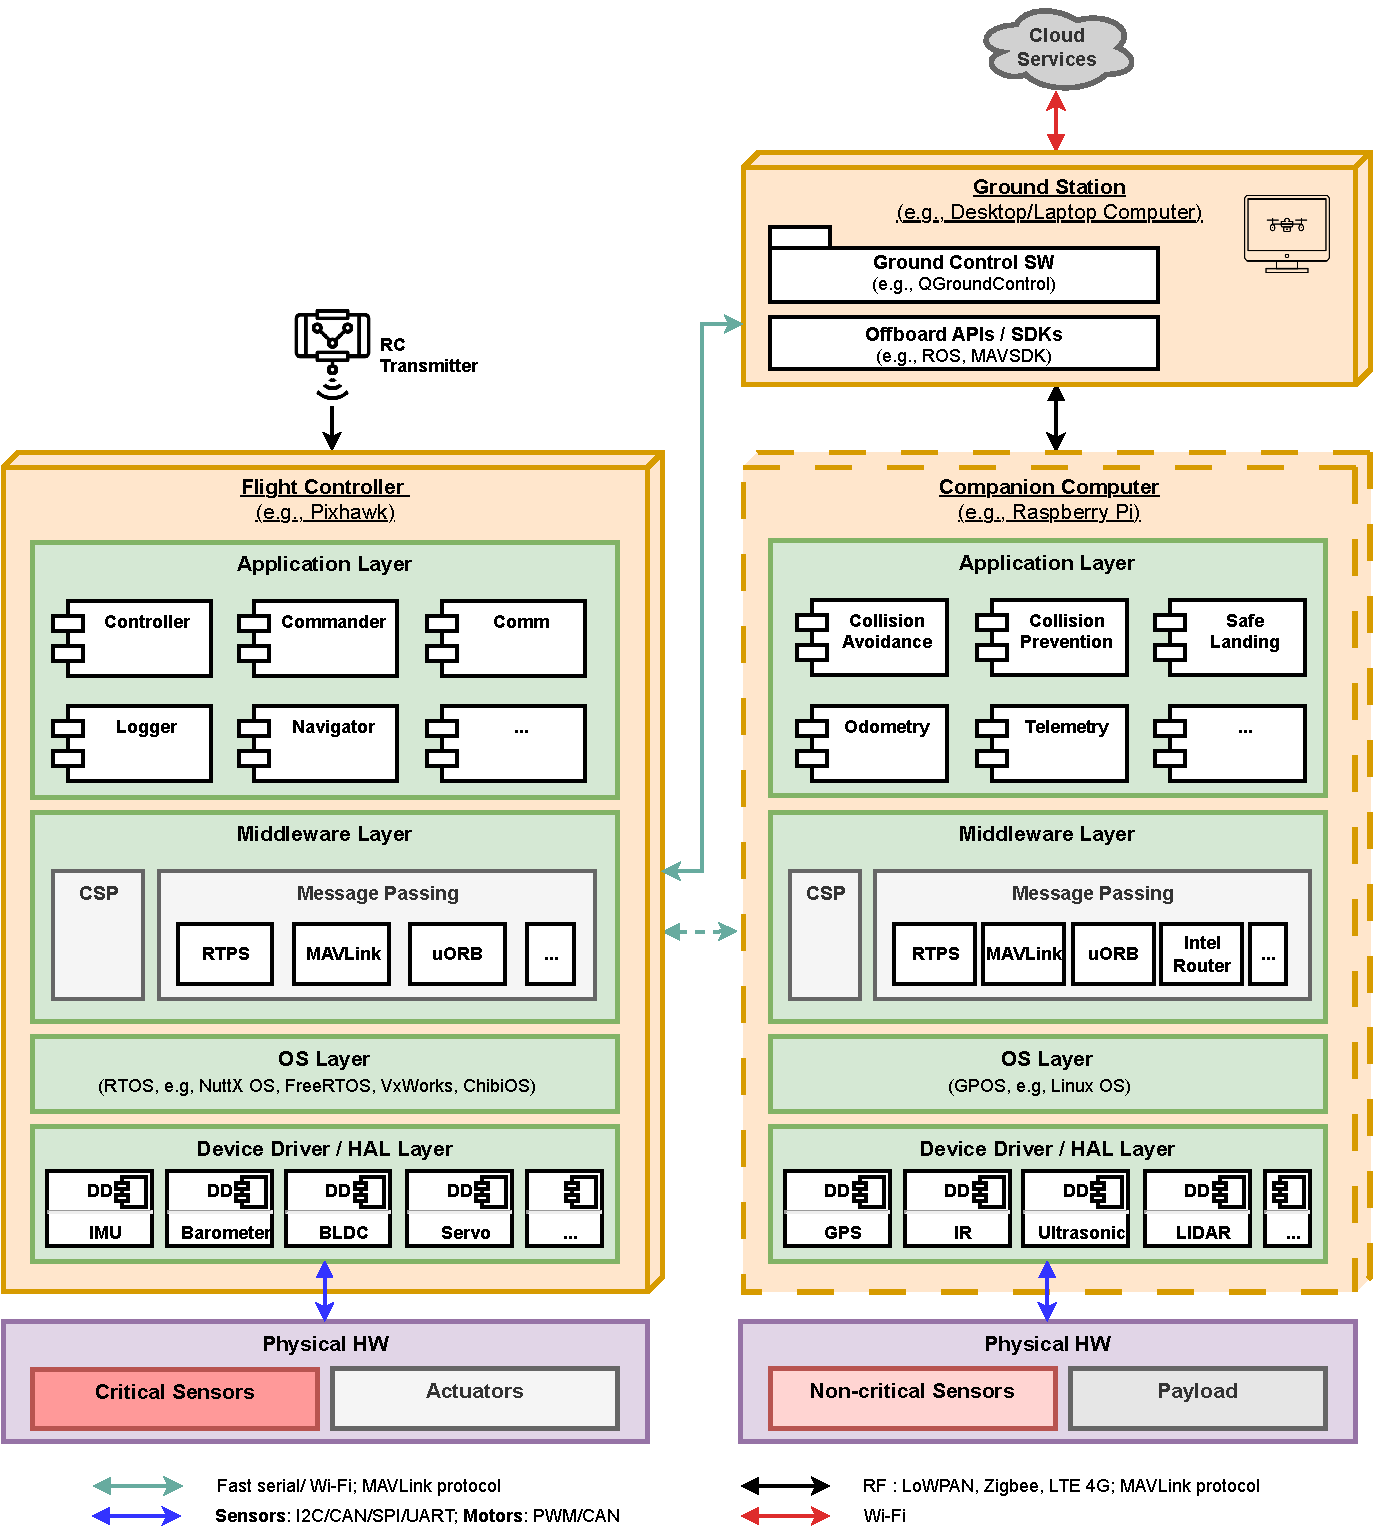
\includegraphics[width=\textwidth]{./img/pdf/uav-sw-arch.pdf}
  \caption{UAV software architecture: common structure}
  \label{fig:uav-sw-arch}
\end{figure}

The software stacks on the flight controller and on the companion computer are structurally similar and commonly organized into four layers:

\begin{enumerate}
\item \textbf{Application layer}: high-level functions of the system. 
      On the flight controller, these are safety-critical tasks, such as \emph{Controller}, \emph{Commander}, \emph{Navigator}, \emph{Logger}, and \emph{Communications}. 
      On the companion computer, secondary tasks provide mission and navigation features, such as \emph{Collision Avoidance}, \emph{Collision Prevention}, \emph{Safe Landing}, \emph{Odometry}, and \emph{Telemetry}.

\item \textbf{Middleware layer}: abstracts the \gls{os} interface and communication via message passing using real-time or asynchronous protocols (e.g., \gls{rtps}, MAVLink, \gls{uorb}). 
      It can also enforce \gls{csp} mechanisms for additional protection. 
      The flight controller typically communicates with the \gls{gcs} over Wi-Fi or other data links and, optionally, with the companion computer via high-throughput serial or Ethernet.

\item \textbf{\gls{os} layer}: provides basic services and a development environment. 
      The flight controller runs an \gls{rtos} (e.g., \lstinline|NuttX|, \lstinline|FreeRTOS|, \lstinline|VxWorks|, \lstinline|ChibiOS|) to meet tight control deadlines. 
      The companion computer runs a \gls{gpos} (typically Linux) because its applications have soft real-time constraints and benefit from the richer software ecosystem (e.g., \gls{ros}-based avoidance libraries for Linux~\cite{px4-sysArch}).

\item \textbf{Device-driver (\gls{hal}) layer}: abstracts the underlying hardware and exposes a stable interface to the \gls{os} for sensor data acquisition and actuator control.
\end{enumerate}

The \gls{gcs} software (e.g., \emph{QGroundControl}) typically runs on a desktop/laptop or mobile device, providing real-time monitoring (often map-overlaid) and flight control. 
Communication can be direct to the flight controller or routed via the companion computer. 
Interfaces between onboard components and the \gls{gcs} commonly use off-board \glspl{api}/\glspl{sdk}, such as \gls{ros} or MAVSDK~\cite{px4-sysArch}.

\subsubsection{Open-source solutions}%
\label{sec:open-source-solut-sw}

\glsxtrfull{oss} platforms, like their hardware counterparts, aim for transparency, flexibility, and maintainability while remaining cost-effective. 
By \gls{oss} we mean that the software source code is released under free/libre terms~\cite{freeGNU}. 
The most prominent open autopilots today are \lstinline|PX4|~\cite{px4-github}, \lstinline|ArduPilot|~\cite{arduPilot-github}, \lstinline|Paparazzi UAS|~\cite{paparazzi-github}, and \lstinline|INAV|. 
Other flight-control firmware -- such as
\lstinline|Betaflight|~\cite{betaflight-github},
\lstinline|Cleanflight|~\cite{cleanflight-github},
\lstinline|Crazyflie|~\cite{crazyflie-home}, and
\lstinline|LibrePilot|~\cite{librePilot-arch} -- targets the \gls{fpv} racing domain and assumes expert manual piloting, so full autopilot features are typically unnecessary and not supported. 
\lstinline|LibrePilot| runs on FreeRTOS but is not actively maintained~\cite{librePilot-github}, whereas \lstinline|Betaflight|, \lstinline|Cleanflight|, and \lstinline|Crazyflie| run directly on the board.

\paragraph{PX4.}
\lstinline|PX4| is an autopilot stack for \glspl{uv}, with a strong focus on \glspl{uav}. 
Started in 2012 and released under a permissive BSD-2-Clause license~\cite{px4-github}, it is widely adopted in industrial and commercial settings~\cite{skynodeX-px4,spRacing-px4}. 
Like ArduPilot, it supports a broad range of \gls{uav} airframes and other vehicles. 
PX4 is flashed onto flight-controller hardware using \emph{QGroundControl} and typically runs atop NuttX; ROS-based workflows are also available~\cite{jargalsaikhan2022architectural}. 
\emph{QGroundControl} configures PX4 and provides the operator interface; an \gls{rc} unit can be used for manual control. 
PX4 uses MAVLink for offboard communication and \gls{uorb} for intra-stack messaging~\cite{px4-sysArch,jargalsaikhan2022architectural}. 
Manual modes require an \gls{imu}, magnetometer, and barometer; autonomous modes also require \gls{gps}. 
Logs are produced on takeoff and can be analyzed with \emph{Flight Review} or \emph{Px4Tools}~\cite{glossner2021overview}.

\paragraph{ArduPilot.}
\lstinline|ArduPilot| is another widely used stack for \glspl{uv}, with strong emphasis on \glspl{uav}. 
Started in 2009 under the GPLv3 license~\cite{arduPilotHistory}, it supports Linux and ChibiOS~\cite{arduPilot-github,jargalsaikhan2022architectural} and runs on many \gls{osh} platforms (e.g., Pixhawk). 
Features -- similar in scope to PX4~\cite{px4-features} -- include multiple flight modes (manual, semi-autonomous, autonomous) with several stabilization options, programmable 3D waypoint missions with optional geofencing, broad sensor and bus support, fail-safes, and navigation in \gls{gps}-denied environments~\cite{arduPilot-home}. 
ArduPilot uses MAVLink to communicate with \glspl{gcs} and companion computers~\cite{arduPilot-home}. 
Mission commands are stored in \gls{eeprom} and executed sequentially in \emph{Auto} mode~\cite{ardupilot-mavlink}.

\paragraph{Paparazzi UAS.}
\lstinline|Paparazzi UAS| is the oldest still-active open autopilot. 
Started in 2003 under GPLv2, it supports multiple \gls{uav}
airframes~\cite{paparazzi-home}.
It runs atop ChibiOS~\cite{paparazzi-sysOverv}, uses \emph{PPRZLINK} for
\gls{gcs} and companion communication~\cite{paparazzi-sysOverv}, and employs the
\emph{AirBorne Ivy} (\gls{abi}) middleware for intra-stack
messaging~\cite{jargalsaikhan2022architectural}.

\paragraph{INAV.}
Derived from \lstinline|Cleanflight|, \lstinline|INAV| targets multirotors,
fixed-wing aircraft, and rovers that need \gls{gps}-assisted flight rather than
acro/racing~\cite{inav-github}.
It sits between racing-oriented \lstinline|Betaflight| and full-autonomy stacks
such as \lstinline|ArduPilot|, providing features like position/altitude hold,
return-to-home, and waypoint missions configured via the
\lstinline|INAV Configurator|~\cite{inav-github}.
Hardware support is limited compared with PX4/ArduPilot, focusing on STM32
F4/F7/H7 and AT32 families~\cite{inav-github}.

\subsubsection{Commercial solutions}%
\label{sec:commercial-solutions-sw}

Commercial proprietary platforms typically disclose limited technical detail. 
Extensibility is offered via vendor \glspl{sdk} (e.g., DJI~\cite{djiSDK}, Parrot~\cite{parrot-sdk}), 
which enable access to additional features but require specialized knowledge.
%
Some vendors also leverage permissive \gls{oss} licenses (e.g., PX4’s BSD) to
add features and ship closed, enterprise-hardened variants.
A representative example is Auterion PX4 (APX4), a hardened PX4 distribution integrated with Auterion \glspl{fmu} and their mission-computer stack. 
Figure~\ref{fig:uav-sw-arch-auterion} sketches the Auterion software architecture.

\begin{figure}[!hbt]
  \centering
  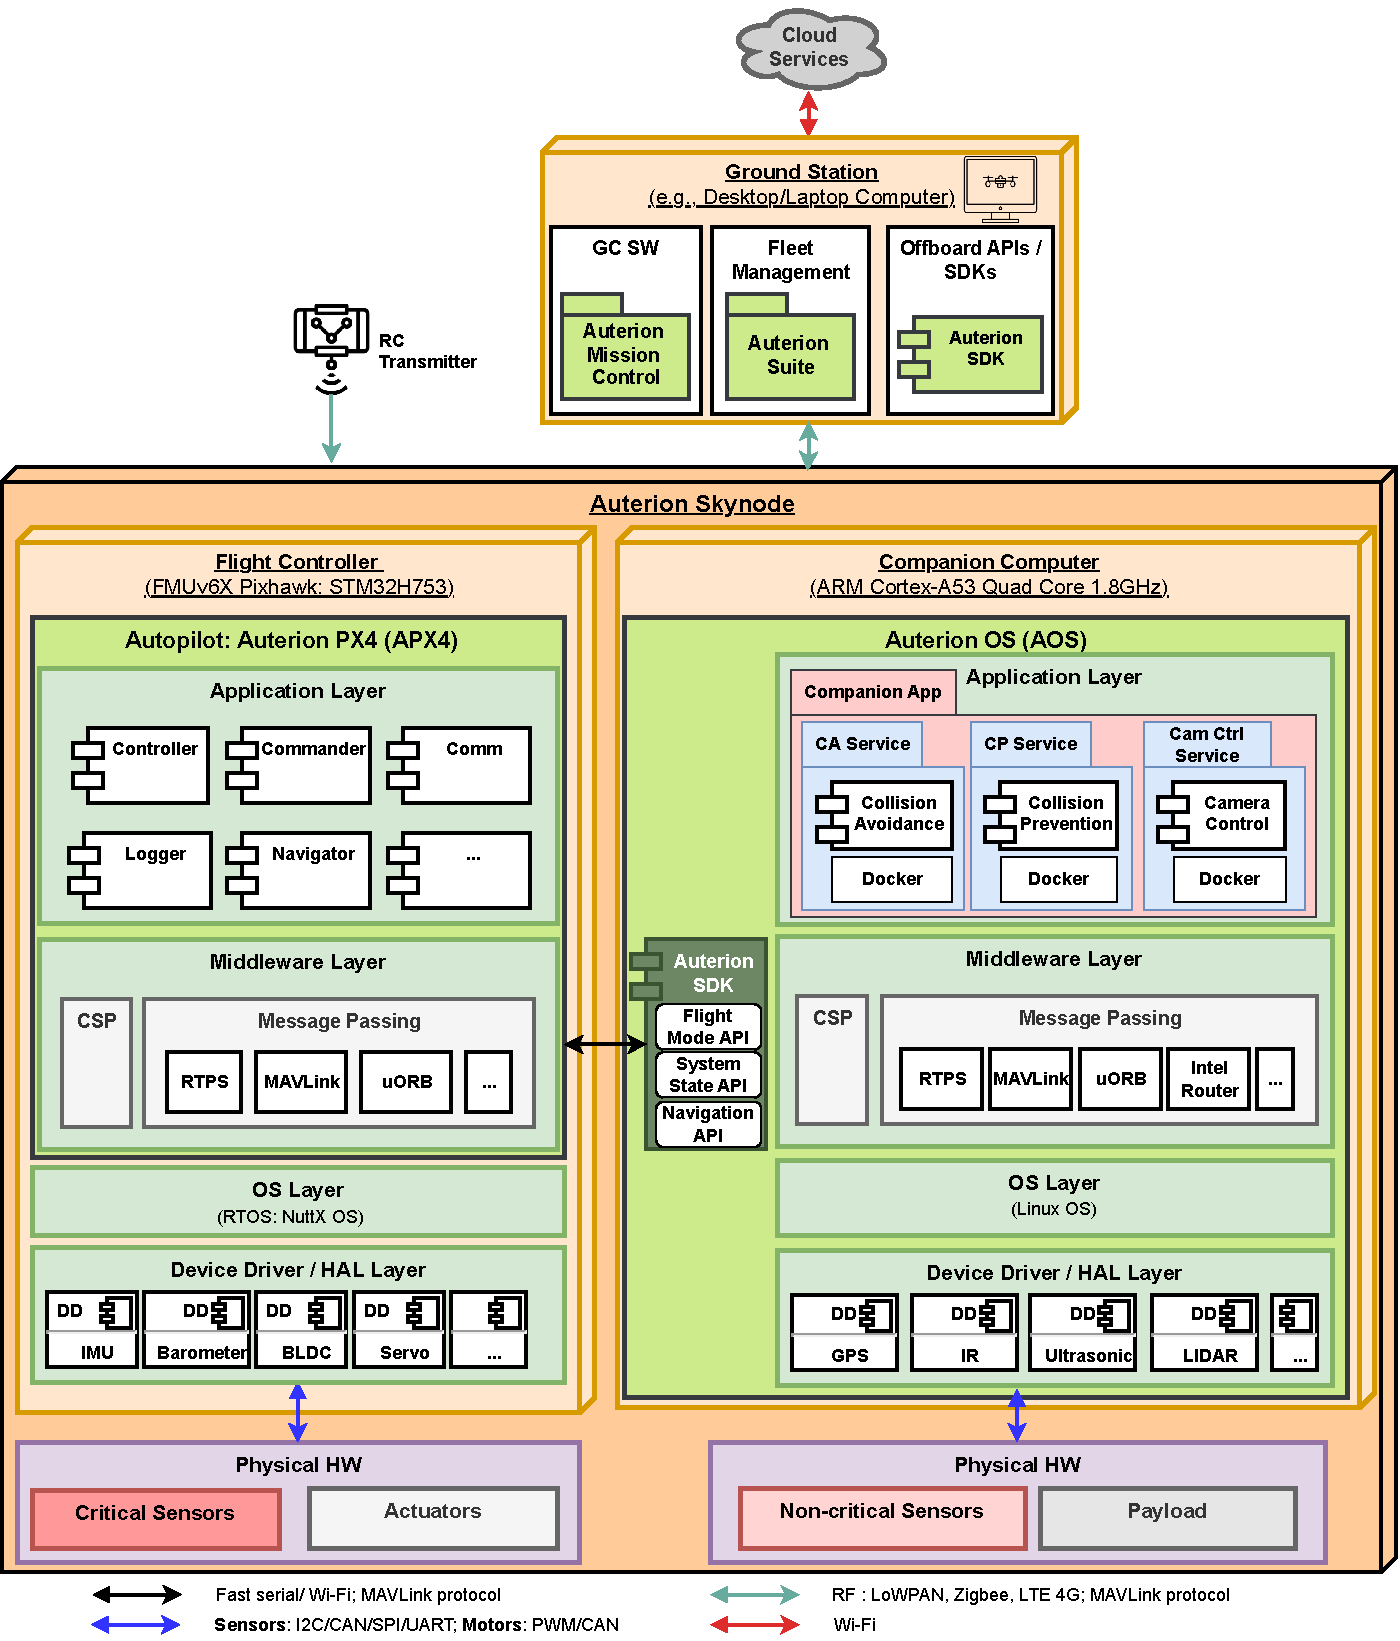
\includegraphics[width=0.9\textwidth]{./img/pdf/uav-main-sw-arch-auterion.pdf}
  \caption{UAV software architecture: Auterion software stack.}
  \label{fig:uav-sw-arch-auterion}
\end{figure}

The \lstinline|Auterion Skynode| co-packages a Pixhawk FMUv6x-based \gls{fmu} and a companion/mission computer on a single board~\cite{auterion-sw}. 
The flight controller runs APX4 (PX4-based) atop NuttX; NuttX is Apache~2.0
licensed, which permits proprietary reuse.
The mission computer runs Auterion~OS (AOS), a customized embedded Linux
distribution that hosts autonomy and payload services (e.g., collision
avoidance, odometry, camera control)~\cite{auterion-sw}.
These services follow a microservices model and are containerized using Docker to improve isolation and streamline updates. 
To reduce storage and update overhead, Auterion recommends: 
(i) packaging related services into a single deployable application (e.g., a \emph{Companion App} distributed as a \lstinline|.auterionos| image), and 
(ii) using a shared base \lstinline|Dockerfile| across services~\cite{auterion-sw-services}. 
Applications interact with the autopilot through the \lstinline|Auterion SDK| \glspl{api}.
%
For control and fleet operations, \emph{Auterion Mission Control} provides a \gls{gcs} tailored to Auterion vehicles~\cite{auterion-missionControl}, 
while \emph{Auterion Suite} offers fleet management, real-time health monitoring, analytics, and \gls{ota} updates~\cite{auterion-suite}. 
Skynode systems may also be operated with a conventional \gls{rc} transmitter or third-party \gls{gcs} software.

If we broaden the view to include any proprietary software component in the stack, 
notably commercial \glspl{rtos} such as \lstinline|VxWorks|, the landscape expands considerably. 
Examples include Northrop Grumman's X-47B~\cite{vxWorks-uav-northrop}, Airbus Helionix~\cite{vxWorks-uav-aribus-helionic}, and Airbus Atlante~\cite{vxWorks-uav-aribus-atlante}.
%
Table~\ref{tab:sw-ref} summarizes the \gls{uav} reference software.


\begin{table}[t]
  \centering
  \caption{UAV reference software summary}
  \label{tab:sw-ref}

  % ---- local-only sizing/spacing ----
  \begingroup
  \footnotesize
  \setlength{\tabcolsep}{4pt}      % tighter column padding
  \renewcommand{\arraystretch}{1.05}% slightly tighter rows

  \begin{tabular}{@{} l l l c l @{}}
    \toprule
    \textbf{FCS} & \textbf{License} & \textbf{OS} & \textbf{Autopilot} & \textbf{Notes} \\
    \midrule
    ArduPilot     & GPL~3        & ChibiOS; Linux & Yes & Autopilot \\
    PX4           & BSD~3        & NuttX; Linux   & Yes & Autopilot \\
    Paparazzi UAS & GPL~2        & ChibiOS        & Yes & Autopilot \\
    INAV          & GPL~3        & Baremetal      & Yes & Autopilot \\
    Crazyflie     & GPL~3        & Baremetal      & No  & Racing \\
    Betaflight    & GPL~3        & Baremetal      & No  & Racing \\
    CleanFlight   & GPL~3        & Baremetal      & No  & Racing \\
    KK2           & GPL~3        & Baremetal      & No  & Not maintained \\
    LibrePilot    & GPL~3        & FreeRTOS       & No  & Not maintained \\
    Dji           & Proprietary  & ND             & Yes & Provides SDK \\
    Parrot        & Proprietary  & ND             & Yes & Provides SDK \\
    APX4          & Proprietary  & NuttX          & Yes & Provides SDK \\
    \bottomrule
  \end{tabular}

  \endgroup
  % ---- local-only sizing/spacing ends ----
\end{table}

% ============================================================================
\section{Related Work}
\label{sec:related-work}
% -- GOAL: Survey what exists for trustworthy UAV software stacks,
%    define how you judge “trustworthy,” summarize current flight stacks + platforms,
%    and review virtualization options used onboard. Finish with a tight gap analysis
%    that bridges to your Design/Implementation.

%============================================================
% Scope and criteria (kept inline as you prefer)
We review prior work on UAV flight stacks, onboard platforms, and virtualization
approaches to understand what is required to safely consolidate mixed-critical
workloads on a single platform.
We focus on deployments where flight-control (safety-critical) and
mission/auxiliary functions (non-critical) must coexist with bounded
interference and predictable timing.
We define \emph{trustworthiness} as the conjunction of: (i) temporal, spatial,
and fault-containment isolation with verifiable real-time behavior; (ii)
deterministic execution and analyzable latency budgets; (iii) a small, auditable
\gls{tcb} and a maintainable codebase; (iv) platform fit under SWaP-C
constraints; and (v) openness to enable scrutiny and broad adoption.
We use these criteria to assess prior work throughout this section.
% Where applicable, we
% interpret these dimensions against sector standards (e.g., DO-178C, ISO 26262)
% and UAV-specific device/timing constraints.


%============================================================
\subsection{Flight Control Software Used in Practice}
\label{subsec:rw-flight-stacks}
The most widely used open-source autopilots are PX4, ArduPilot, Paparazzi UAS,
and INAV.
PX4, widely adopted in industrial and commercial settings, runs on NuttX (and
Linux), offers broad platform coverage, and has a modular architecture.
ArduPilot targets Linux and ChibiOS, with extensive support for \gls{osh}
platforms (e.g., Pixhawk) and rich vehicle types.
Paparazzi UAS, one of the earliest open stacks, runs atop ChibiOS with a strong
fixed-wing heritage.
INAV sits between racing firmware (e.g., Betaflight) and full autopilots,
emphasizing GPS-assisted flight but supporting only a subset of boards (notably
STM32 F4/F7/H7 and AT32).

Jargalsaikhan et al.~\cite{jargalsaikhan2022architectural} analyzed module-level
portability across PX4, ArduPilot, Paparazzi, and a custom stack, evaluating
structure, messaging, and \gls{hal} design against portability requirements
(simplicity, modularity, centralized messaging, standard interfaces, \gls{hal}
quality, documentation). They found that only \emph{ArduPilot} and \emph{PX4}
provide \glspl{hal} and that \emph{ArduPilot} lacks message
centralization. Moreover, all surveyed systems rely on non-standard messaging,
which hinders portability despite being open source.

In 2021, Wang et al.~\cite{wang_exploratory_2021} conducted an exploratory study
of autopilot software bugs, analyzing 569 fixed issues from PX4 and ArduPilot
and identifying 168 UAV-specific bugs. Root causes spanned eight classes (e.g.,
missing initialization, limit/parameter mishandling, hardware/software-dependent
priority), highlighting recurring pain points. They reported that 39\% of those
bugs pertained to PX4 (with \(\approx\)609~kLOC) versus ArduPilot (\(>1505\)~kLOC), and
that PX4 had more resolved issues overall (\(\approx\)5k vs.\ \(\approx\)3.5k), suggesting
a highly engaged community. Such scrutiny is only possible with open-source
stacks, improving transparency and, by extension, trustworthiness.

Much academic work with PX4 and ArduPilot targets flight
control~\cite{li_embedding_2022,li_plug-and-play_2021,baldi_ardupilot-based_2022,dangelo_efficient_2024}
and simulation-based
verification~\cite{baldi_ardupilot-based_2022,dang_nguyen_vision-based_2019,dai_rflysim_2021},
often to develop adaptive control and to broaden functional test coverage via
\gls{sitl}/\gls{hitl}.
D'Angelo et al.~\cite{dangelo_efficient_2024} explicitly cite PX4's BSD-3
license as enabling code modifications without mandatory upstreaming, helping
companies protect intellectual property.
%

In the commercial domain, flight-control software is typically closed-source,
with extensibility exposed via \glspl{sdk}~\cite{parrot-sdk}. Auterion, by
contrast, maintains a proprietary PX4 fork for the flight controller and deploys mission applications via containers on the companion computer. % NOTE: brief here; full discussion appears later
%
Buquerin~\cite{buquerin2018security} evaluated the
VxWorks~7 \gls{rtos} (commercial, avionics) and reported that basic attacks (e.g., buffer overflows, string vulnerabilities) caused noticeable performance degradation, with no built-in protection against malware or command injection.
This underscores the need for supervising technology (e.g., a hypervisor) to contain faults across domains.

With open-source \glspl{rtos}, transparency increases but isolation is still limited.
Zhang et al.~\cite{zhang2021best} compared NuttX and ChibiOS: ChibiOS generally
outperformed NuttX on timing, avoided priority inversion with mutexes, and
exhibited lower context-switch overhead; NuttX lacks priority inheritance with
mutexes and has a larger codebase.
Thus, an \gls{rtos} alone does not provide the inter-domain isolation required for \glspl{mcs}.

From a mixed-criticality perspective, PX4 and ArduPilot emerge as the most
mature and widely supported open-source autopilots, but non-standard messaging and large codebases
complicate portability and assurance. Paparazzi remains influential historically
yet narrower in scope, while INAV targets GPS-assisted use cases on a limited
set of boards. Openness consistently improves auditability and community
response, but real-time determinism and isolation depend on the underlying \gls{os}
(NuttX/ChibiOS/Linux) and on supervisory mechanisms (e.g., hypervisors).
Because none of these stacks alone provide strong inter-domain isolation, we
next examine the hardware platforms and hypervisor-based partitioning for mixed-critical deployments.

%============================================================
\subsection{Hardware Platforms for Onboard Integration}
\label{subsec:rw-hw-context}
Common architectures fall into three categories.
First, a dedicated \gls{fmu} (running the autopilot) paired with a companion
computer for mission functions~\cite{pixhawk4,arduPilot-cuavV5}. Some products
co-package both (e.g., PixC4–Jetson~\cite{jetson-docs}) yet still communicate
over external links (often \gls{uart}).
%
Second, single-board Linux systems with add-on shields merge flight control and
mission functions on one \gls{soc} (e.g., Navio2~\cite{navio2-px4},
PilotPi~\cite{px4-pilotpi} on Raspberry Pi), trading strong isolation for
availability and cost. To consolidate critical and non-critical stacks on a
shared \gls{hw} platform, a resource-efficient and secure mechanism is
needed -- typically a hypervisor with disciplined device assignment.

Third, heterogeneous FPGA+\gls{soc} platforms integrate high-performance
application processing with accelerated I/O or perception. The Aerotenna
OcPoC-Zynq Mini, currently discontinued, ~\cite{ocpoc,ocpoc-discontinued} combined dual-core Cortex-A9
Linux with an Artix-7 \gls{fpga} for extended sensors and I/O, running PX4 or
ArduPilot. In academia, Kovari and Ebeid~\cite{kovari_mpdrone_2021} used an
Avnet Ultra96-V2 (Zynq UltraScale+ MPSoC) with \gls{ros} on the \gls{cpu} (OpenCV) and
YOLOv3 offloaded to the \gls{fpga}, while PX4 remained on an external
Pixhawk, illustrating that the mixed-criticality stacks were not consolidated
onto the same platform. Cittadini et al.~\cite{cittadini_supporting_2023}
implemented a two-domain stack on a Zynq UltraScale+: Linux (three cores) runs a
YOLOv3 pipeline on an accelerator while a FreeRTOS domain handles low-level
control atop the static-partitioning hypervisor CLARE~\cite{clare-home}.
However, CLARE is closed-source and the flight stack was tailored, limiting
scalability.

A complementary approach is to use heterogeneous \glspl{soc} that host Linux on
high-performance cores and an \gls{rtos} on real-time cores, promising cleaner
separation with lower \gls{swap-c} if toolchains and hypervisors are
mature. Valente et al.~\cite{valente_heterogeneous_2024} exemplify this with
\emph{Shaheen}, a RISC-V heterogeneous SoC (RV64 host + RV32 cluster) enabling
\gls{rtos}+Linux co-existence under nano-\gls{uav} power budgets via the Bao hypervisor. % NOTE: “the Bao”
To our knowledge, this is the only open-standards heterogeneous platform explicitly
targeting \gls{uav} stack consolidation to date.
%
This context motivates the hypervisor-based partitioning survey below: a small,
analyzable \gls{tcb} that can deliver strong spatial, temporal, and fault
isolation while fitting SWaP-C budgets.

%============================================================
\subsection{Virtualization for Onboard Mixed-Criticality}
\label{subsec:rw-virt}
Wang et al.~\cite{wang_enabling_2018} analyzed container- and KVM-based
virtualization on Arm \glspl{soc} (e.g., Jetson TX2). KVM (with vGIC/QEMU) provides VM-level isolation via
trap-and-emulate and two-stage address translation, whereas containers rely on
Linux namespaces and cgroups (shared kernel).
Experiments show containers are closer to native for compute and
network throughput, while KVM provides stronger kernel isolation and remains
resilient under fork-bomb stress. % NOTE: moved Auterion elaboration out of stacks; keep it here:
Auterion deploys mission applications in containers on the companion computer~\cite{auterion-sw-services}.
However, because containers share a kernel, they cannot by themselves enforce strong separation for mixed-critical workloads.

Virtualization provides isolation properties that containerization cannot:
temporal isolation (bounded interference), spatial isolation (memory and device
protection), and fault containment across \glspl{vm}. Containers share a host
kernel and therefore cannot, by themselves, meet strong separation requirements
for mixed-criticality workloads.

Fautrel et al.~\cite{fautrel_hypervisor_2019} advocate a type-1 hypervisor with
two-level scheduling: \glspl{vm} are scheduled first with fixed period/slot
windows, and tasks in each \gls{vm} use fixed task priority. They provide
schedulability conditions, minimum and maximum \gls{vm}-period bounds accounting
for context-switch overhead, and an algorithm to compute feasible \gls{vm}
periods and slots to meet all tasks' deadlines.
To validate the algorithm, the authors use an inspection drone system comprising
three mixed-criticality \glspl{vm}: (1) high -- autopilot on bare metal; (2)
medium -- \gls{gcs}-\gls{uav} communications on OpenWRT; and (3) low -- video processing on
Debian Linux.
The authors advocated PikeOS Level~1 as a DO-178B/C-certifiable option for airborne systems,
but PikeOS~\cite{pikeOS} is closed source, limiting adoption in low-cost \glspl{uav}.
Cittadini et al.~\cite{cittadini_supporting_2023} similarly used the closed-source
CLARE hypervisor to implement a two-domain \gls{uav} stack. With static allocation and \gls{fpga} pass-through, they reported near-zero overhead
relative to a non-hypervisor (bare-metal) baseline and µs–ms shared-memory latencies.

Klein et al.~\cite{klein_formally_2018} used the open-source seL4 microkernel combined with
the CAmkES \gls{vmm} to deploy two \glspl{vm} on the mission computer: a
non-critical Linux guest for camera and Wi-Fi; and a critical bare-metal
application handling \gls{can}-over-Ethernet communications and cryptography.
However, the threat model excludes radio-frequency jamming/\gls{dos} on the \gls{gcs}
link and assumes a correct, uncompromised autopilot. These are strong
assumptions given known bug densities in open-source
autopilots~\cite{wang_exploratory_2021} and vulnerabilities in commercial \glspl{rtos}~\cite{buquerin2018security}.

Farrukh and West~\cite{farrukh_flyos_2023} presented FlyOS, an architecture
that consolidates critical and non-critical stacks on a heterogeneous multicore
platform: the non-critical stack runs in a Linux \gls{vm}, while the critical
stack runs in the Quest \gls{rtos}~\cite{danish_virtual-cpu_2011,questOS-home,questOS-repo}.
Both \glspl{vm} execute atop the Quest-V separation-kernel
hypervisor~\cite{li_quest-v_2013}. The authors tailored Cleanflight to the
application's needs and used shared memory to send mission commands from the
Linux \gls{vm} to the critical \gls{vm}. They added fault tolerance via
\gls{vm}-level redundancy (heartbeat monitoring and re-instantiation).
The prototype targets the Intel Aero Compute Board (now deprecated)~\cite{intel-aero}.
While compelling, the design has limitations: (1) customizing the flight-control
firmware reduces portability; (2) because Cleanflight is not a full autopilot, the Linux guest must continuously compute and emit
setpoints; (3) and Quest OS currently supports only x86~\cite{questOS-home}
and, despite being open-source, is unmaintained~\cite{questOS-repo}, which
weakens trustworthiness.

Valente et al.~\cite{valente_heterogeneous_2024} followed a complementary approach:
when designing a heterogeneous RISC-V \gls{soc} for secure nano-\glspl{uav}, they advocated the Bao hypervisor as the key element
to isolate mixed-critical stacks. By design, this attests to the centrality of
hypervisor-based isolation in \gls{uav} consolidation.

\subsection{Synthesis and Gap Analysis}
\label{subsec:rw-gap}
Table~\ref{tab:rw-compare} compares representative systems against
consolidation-relevant criteria for \glspl{uav}.

\begin{table}[!tbp]
  \centering
  \caption{Prior systems vs.\ consolidation-relevant criteria (UAV focus)}
  \label{tab:rw-compare}
  \begingroup
  \setlength{\tabcolsep}{3.2pt}
  \renewcommand{\arraystretch}{1.10}
  \setlength{\extrarowheight}{0.4ex}
  \scriptsize
  \begin{tabularx}{\textwidth}{@{}%
    >{\raggedright\arraybackslash}p{1.8cm}  % System/Work
    >{\centering\arraybackslash}p{0.9cm}    % Open?
    >{\raggedright\arraybackslash}p{3.0cm}  % Isolation model
    >{\raggedright\arraybackslash}p{3.0cm}  % RT evidence
    >{\raggedright\arraybackslash}p{2.1cm}  % TCB (qual.)
    >{\raggedright\arraybackslash}p{1.5cm}  % Platform
    >{\raggedright\arraybackslash}X         % UAV status / Refs.
    @{}}
    \toprule
    \textbf{System/Work} & \textbf{Open?} & \textbf{Isolation model} & \textbf{RT evidence} & \textbf{TCB} & \textbf{Platform} & \textbf{Notes} \\
    \midrule
    FMU + Companion (no HV) & — & \textit{Board separation} (no virtualization); autopilot on dedicated FCU; missions on companion & FCU RT via PX4/ArduPilot/RTOS; isolation by hardware boundary & Split across boards (small FCU RTOS; larger companion OS) & Pixhawk + Jetson/RPi (typical) & Widely deployed; e.g., Pixhawk~4, PixC4–Jetson \cite{pixhawk4,jetson-docs} \\
    \midrule
    Docker vs.\ KVM on TX2 \cite{wang_enabling_2018} & — & Containers (shared kernel) vs.\ KVM VMs & Throughput + stress; containers \(\approx\) native; KVM resilient to fork-bomb & KVM larger; containers share kernel & Jetson TX2 (Arm) & Mission-computer study \\
    Two-level sched.\ \cite{fautrel_hypervisor_2019} & — & Type-1 static; VM time slots + fixed-priority tasks & Schedulability bounds incl.\ context-switch cost & HV-dependent & Generic (Arm) & Algorithms validated on UAV inspection prototype \\
    PikeOS~\cite{pikeOS}  & No & ARINC-653 time/space partitions (table-based) & Certified RT services; partition slots & Mid/High & Arm (var.) & Industrial/avionics deployments \\
    seL4 + CAmkES VMM \cite{klein_formally_2018} & Yes & Microkernel + VMM; native components + Linux VM & Kernel proofs; containment demo on UAV & Very small (verified kernel) & Arm & Virtualization on mission computer only; unconsolidated HW \\
    FlyOS + Quest-V~\cite{farrukh_flyos_2023} & Partial & Separation-kernel VMs (Linux + Quest RT) & Fault tolerance (VM heartbeat/restore) & Mid (kernel+guests) & Intel Aero (x86) & Custom Cleanflight-based firmware; maintenance status unclear \\
    CLARE on ZCU104 \cite{cittadini_supporting_2023} & Partial (HV) & Type-1 static; Linux (AI) + FreeRTOS (control) & Near-zero HV overhead; \(\mu s\)–\(ms\) cross-domain; \(\sim\)10\,ms fail-safe & Mid (HV+OSes) & Zynq US+ MPSoC & UAV tracking demo \\
    Shaheen SoC~\cite{valente_heterogeneous_2024} & Yes & HW virt (RISC-V H-ext) + Bao-style static partitions & Power/throughput + timing-channel controls & Small HV + SoC IPs & RV64 host + RV32 cluster & Nano-UAV silicon platform \\
    Bao (static partitioner) & Yes & Type-1, static; 1:1 vCPU:pCPU; static memory; cache coloring & Embedded benchmarks; low HV overhead & Small (\(\sim\)8k C + \(\sim\)0.5k asm) & Armv7/8-A/-R; RISC-V & Basis for mixed-critical stacks \cite{martins_et_al:OASIcs:2020:11779,baoRepo,martins2023shedding} \\
    \bottomrule
  \end{tabularx}
  \endgroup
\end{table}

The conventional \emph{\gls{fmu} + companion} split provides strong fault isolation by hardware separation, but incurs \gls{swap-c} costs and introduces latency/bandwidth limits across board boundaries.
Containerization helps package mission software but shares a kernel and thus
cannot, by itself, enforce strong temporal/spatial isolation.
Hypervisor-based partitioning emerges as the practical path to consolidate
mixed-critical workloads on one platform; within this space, static-partitioning
hypervisors (e.g., Bao) are attractive due to small \glspl{tcb}, 1:1 vCPU:pCPU
mapping, pass-through \gls{io}, and reliance on two-stage translation for
memory/device isolation.


Two cross-cutting gaps remain: \emph{trustworthiness} and \emph{openness}.
Industrial-grade options like PikeOS and CLARE are not open-source, limiting transparency and community audit.
seL4 + CAmkES VMM demonstrations typically protect the mission computer while leaving the flight controller off-board, i.e., without full consolidation on a single \gls{soc}.
FlyOS/Quest-V shows an integrated design but depends on x86-only, unmaintained components and a customized flight stack, which constrains portability.
These gaps motivate a trustworthy, open solution with a small auditable \gls{tcb} and static partitioning on accessible hardware.
In this context, Bao provides a suitable foundation, following the
footsteps of the Shaheen heterogeneous
\gls{soc}\cite{valente_heterogeneous_2024} premises for nano-\gls{uav}
applications: static partitioning plus carefully selected device assignment can
meet \gls{swap-c} budgets while preserving isolation.
Given the SWaP-C, openness, and isolation requirements, we adopt Bao for
enabling the consolidation of mixed-criticality software stacks in \gls{uav} applications.


% %============================================================

% END Related Work
%%% Local Variables:
%%% mode: latex
%%% TeX-master: "../template"
%%% reftex-default-bibliography: ("../Bibliography/mieeic.bib")
%%% ispell-local-dictionary: "american"
%%% End:
